% -*- coding: utf-8 -*-

\begin{chapter}{Прибрежные процессы и~приливные явления}\label{chap:17}
% \chapter{Coastal Processes and Tides} 
В предыдущей главе мы рассматривали волны на поверхности океана в целом,
а сейчас обратимся к некоторым важным частным случаям, таким как
трансформация и разрушение волн при подходе к побережью, 
течения и краевые волны, возникающие в результате взаимодействия волн 
с берегом, цунами\index{цунами}, штормовые нагоны и, наконец, 
приливные явления, происходящие как у побережья, так и в открытом океане.
%
% In the last chapter I described waves on the sea surface. Now we can
% consider several special and important cases: the transformation of
% waves as they come ashore and break; the currents and edge waves
% generated by the interaction of waves with coasts;
% tsunamis\index{tsunami}; storm surges; and tides, especially tides
% along coasts and in the deep ocean.

\begin{section}{Shoaling Waves и прибрежные процессы}
% \section{Shoaling Waves and Coastal Processes}
\index{волны!shoaling}Фаза волны и групповые скорости зависят от глубины,
если она составляет менее одной четверти длины волны в глубокой воде.
В то же время, период волны и её частота инвариантны (не изменяются при 
подходе к берегу); это свойство используется при расчётах характеристик
прибрежных волн. Высота волны увеличивается при уменьшении групповой скорости,
а длина уменьшается. Направление волн меняется вследствие рефракции. 
И, наконец, при уменьшении глубины до некоторого значения, 
волны разрушаются, а вода, которую они перенесли в зону прибоя, образует
long-shore и разрывные течения\index{разрывные течения}.
%
% \index{waves!shoaling}Wave phase and group velocities are a function
% of depth when the depth is less than about one-quarter wavelength in
% deep water. Wave period and frequency are invariant (don't change as
% the wave comes ashore); and this is used to compute the properties of
% shoaling waves. Wave height increases as wave group velocity
% slows. Wave length decreases. Waves change direction due to
% refraction. Finally, waves break if the water is sufficiently shallow;
% and broken waves pour water into the surf zone, creating long-shore
% and rip currents\index{rip currents}.

\begin{paragraph}{Прибрежные волны.}
% \paragraph{Shoaling Waves}
Дисперсионное соотношение~(\ref{eq:16.3}) используется для расчёта свойств
волны, которая распространяется от глубоководных районов к мелководью
вне зоны прибоя. Так как циклическая частота~$\omega$ постоянна, 
согласно~(\ref{eq:16.3}) получим
\begin{equation}\label{eq:intermed}
 \frac{L}{L_{0}} = \frac{c}{c_{0}}=\frac{\sin \alpha }{\sin \alpha _{0}} 
                 = \Tanh \frac{2 \pi d}{L}, 
\end{equation}
где
\begin{equation}\label{eq:Lzero}
 L_{0} = \frac{g T^{2}}{2 \pi }, \qquad 
 c_{0} = \frac{g T}{2 \pi }, 
\end{equation}
$L$~--- длина волны, $c$~--- фазовая скорость, $\alpha $~--- угол
между гребнем и изобатами, $d$~--- глубина моря. Индексом~$0$
обозначены характеристики в глубокой воде.
%
% The dispersion relation (16.3) is used to calculate wave properties as
% the waves propagate from deep water offshore to shallow water just
% outside the surf zone. Because $\omega$ is constant, (16.3) leads to:
% \begin{equation}
% \frac{L}{L_{0}} = \frac{c}{c_{0}}=\frac{\sin \alpha }{\sin \alpha _{0}} = \tanh
% \frac{2 \pi d}{L} \label{eq:intermed}
% \end{equation}
% where
% \begin{equation}
% L_{0} = \frac{g T^{2}}{2 \pi }, \qquad c_{0} = \frac{g T}{2 \pi } \label{eq:Lzero}
% \end{equation}
% and $L$ is wave length, $c$ is phase velocity, $\alpha $ is the angle
% of the crest relative to contours of constant depth, and $d$ is water
% depth. The subscript $0$ indicates values in deep water.

Чтобы найти величину~$d/L$, решим итерационным методом уравнение
\begin{equation}\label{eq:intermediate}
 \frac{d}{L_{0}} = \frac{d}{L} \Tanh \frac{2 \pi d}{L} 
\end{equation}
либо воспользуемся рис.~\ref{wiegelgraph} или таблицей~A1 
Вейгеля~\cite{Wiegel:1964}.
%
% The quantity $d/L$ is calculated from the solution of
% \begin{equation}
% \frac{d}{L_{0}} = \frac{d}{L} \tanh \frac{2 \pi d}{L} \label{eq:intermediate}
% \end{equation}
% using an iterative technique, or from figure 17.1, or from Wiegel (1964: A1).

\begin{figure}[t!]
\makebox[121 mm] [c]{\includegraphics{pics/wiegelgraph}}
\caption{Свойства волн на глубинах, промежуточных между глубокой и мелкой 
водой. Обозначения: $d$~--- глубина, $L$~--- длина волны, $C$~--- фазовая
скорость, $C_g$~--- групповая скорость, $\alpha$~--- угол между гребнями
волн и линиями постоянной глубины, $H$~--- высота волны. 
Индексом~$0$ обозначены характеристики в глубокой 
воде.~\cite[табл.~A1]{Wiegel:1964}}
\label{wiegelgraph}
\end{figure}
%
% \begin{figure}[t!]
% %\centering
% \makebox[121 mm] [c]{\includegraphics{wiegelgraph}}
% \footnotesize
% Figure 17.1 Properties of \rule{0mm}{3ex}waves in intermediate depths
% between deep and shallow water. $d=$ depth, $L=$ wavelength, $C=$
% phase velocity, $C_g=$ group velocity, $\alpha = $ angle of crests
% relative to contours of constant depth, $H = $ wave height. Subscript
% $0$ refers to properties in deep water. From values in Wiegel (1964:
% A1).
%
% \label{wiegelgraph}
% \vspace{-4ex}
% \end{figure}

\begin{figure}[b!]
\begin{centering}
\makebox[121 mm] [c]{\includegraphics{pics/wavefocusing}}
\end{centering}
\caption{Элементы рельефа дна, такие как подводные каньоны и хребты,
расположенные у побережья, могут существенно повлиять на высоту 
breakers\index{breakers!height of} inshore of the features.~\cite[стр.~229]{Thurman:1985}} 
%% breakers = прибоя???
\label{wavefocusing}
\end{figure}
%
% \begin{figure}[b!]
% \vspace{-1ex}
% \centering
% \makebox[121 mm] [c]{\includegraphics{wavefocusing}}
% \footnotesize
% Figure 17.2 sub-sea \rule{0mm}{4ex}features, such as submarine canyons
% and ridges, offshore of coasts can greatly influence the height of
% breakers\index{breakers!height of} inshore of the features. After
% Thurman (1985: 229).
%
% \label{wavefocusing}
% %\vspace{-2ex}
% \end{figure}

Так как скорость волны в мелкой воде зависит от глубины,
изменение глубины при подходе волны к берегу может сконцентрировать или
рассеять её энергию. Рассмотрим простой случай, когда гребни волн 
в глубокой воде почти параллельны берегу с двумя выступающими в море ridges
%% мысами --- ridges
(рис.~\ref{wavefocusing}). Групповая скорость волн выше
в глубокой части между ridges, так что гребни волн начинают деформироваться
%% ridges --- отмелями
по мере приближения к берегу. Энергия волны, распространяясь
перпендикулярно гребню волны, направляется в сторону мысов, где 
breakers\index{breakers!height of} становятся гораздо сильнее, чем в заливе. 
Различия в высоте волн могут оказаться необычайно большими. Так, в спокойный 
день shoreward of a submarine canyon на пляже Ла-Холья (Калифорния), 
примыкающем с юга к Институту океанографии им. Скриппса, 
breakers могут быть высотой по колено. В то же самое время немного севернее
каньона волны могут быть достаточно высокими, чтобы заинтересовать
любителей сёрфинга.
%
% Because wave velocity is a function of depth in shallow water,
% variations in offshore water depth can focus or defocus wave energy
% reaching the shore. Consider the simple case of waves with deep-water
% crests almost parallel to a straight beach with two ridges each
% extending seaward from a headland (figure 17.2). Wave group velocity
% is faster in the deeper water between the ridges, and the wave crests
% become progressively deformed as the wave propagates toward the
% beach. Wave energy, which propagates perpendicular to wave crests, is
% refracted out of the region between the headland. As a result, wave
% energy is focused into the headlands, and
% breakers\index{breakers!height of} there are much larger than breakers
% in the bay. The difference in wave height can be surprisingly
% large. On a calm day, breakers can be knee high shoreward of a
% submarine canyon at La Jolla Shores, California, just south of the
% Scripps Institution of Oceanography. At the same time, waves just
% north of the canyon can be high enough to attract surfers.
\end{paragraph}

\begin{figure}[t!]
\begin{centering}
\makebox[121 mm] [c]{\includegraphics{pics/breakers}}
\end{centering}
\caption{\textbf{Слева:} классификация\index{breakers!types of} 
разрушающихся волн в зависимости от уклона дна и крутизны волны. 
\textbf{Справа:} схематическое изображение типов разрушающихся 
волн.~\cite[стр.~79, 81]{Horikawa:1988}}
\label{fig:breakers}
\end{figure}
%
% \begin{figure}[t!]
% \centering
% \makebox[121 mm] [c]{\includegraphics{breakers}}
% \footnotesize
% Figure 17.3 \textbf{Left}:
% \rule{0mm}{3ex}Classification\index{breakers!types of} of breaking
% waves as a function of beach steepness and wave steepness
% offshore. \textbf{Right}: Sketch of types of breaking waves. After
% Horikawa (1988: 79, 81).
%
% \label{fig:breakers}
% \vspace{-3ex}
% \end{figure}

\begin{paragraph}{Разрушение волн.}
% \paragraph{Breaking Waves}
\index{волны!разрушение}При движении волн на мелководье их групповая скорость 
уменьшается, энергия на квадратный метр поверхности моря увеличивается, 
а вклад нелинейных членов волновых уравнений становится существенным. 
В результате
волны начинают расти, приобретая вид узких крутых гребней с широкими
мелкими углублениями перед ними.
Когда крутизна волны становится достаточно большой,
волна разрушается (рис.~\ref{fig:breakers}, слева). Форма разрушающейся волны
зависит от уклона дна и крутизны волны при подходе к берегу 
(рис.~\ref{fig:breakers}, справа).
%
% \index{waves!breaking}As waves move into shallow water, the group
% velocity becomes small, wave energy per square meter of sea surface
% increases, and non-linear terms in the wave equations become
% important. These processes cause waves to steepen, with short steep
% crests and broad shallow troughs. When wave slope at the crest becomes
% sufficiently steep, the wave breaks (figure 17.3 Right). The shape of
% the breaking wave depends on the slope of the bottom, and the
% steepness of waves offshore (figure 17.3 Left).
%
\begin{enumerate}
\item 
Крутые волны, как правило, теряют энергию медленно, по мере того, как волны
распространяются в направлении более мелкой воды, за счет стекания воды
по front of the wave. 
These are spilling breakers\index{breakers!spilling}.
%
% \vitem Steep waves tend to lose energy slowly as the waves moves into
% shallower water through water spilling down the front of the
% wave. These are spilling breakers\index{breakers!spilling}.

\item
Менее крутые волны на крутых beaches обычно увеличивают свою крутизну
так быстро, что гребень волны движется намного быстрее углубления, 
вследствие чего гребень нависает над углублением и обрушивается 
в него\index{breakers!plunging} (рис.~\ref{fig:wavecropped}).
%
% \vitem Less steep waves on steep beaches tend to steepen so quickly
% that the crest of the wave moves much faster than the trough, and the
% crest, racing ahead of the trough, plunges\index{breakers!plunging}
% into the trough (figure 17.4).

\item
Если крутизна beach достаточно велика, the wave can
surge\index{breakers!surging} up the face of the beach without
breaking in the sense that white water is formed. Or if it is formed,
it is at the leading edge of the water as it surges up the beach. An
extreme example would be a wave incident on a vertical breakwater.
%
% \vitem If the beach is sufficiently steep, the wave can
% surge\index{breakers!surging} up the face of the beach without
% breaking in the sense that white water is formed. Or if it is formed,
% it is at the leading edge of the water as it surges up the beach. An
% extreme example would be a wave incident on a vertical breakwater.
\end{enumerate}
\end{paragraph}

\begin{figure}[t!]
\makebox[121 mm] [c]{\includegraphics{pics/wavecropped}}
\caption{Крутые plunging breakers\index{breakers!plunging} представляют
собой archetypical breaker. The edge of such breakers идеальны для занятий
сёрфингом. (Фотография Jeff Devine.)}
\label{fig:wavecropped}
\end{figure}
%
% \begin{figure}[t!]
% \makebox[121 mm] [c]{\includegraphics{wavecropped}}
% \centering
% \footnotesize
% Figure 17.4 Steep, plunging
% \rule{0pt}{4ex}breakers\index{breakers!plunging} are the archetypical
% breaker. The edge\\of such breakers are ideal for surfing. From photo
% by Jeff Devine.
%
% \label{fig:wavecropped}
% \vspace{-3ex}
% \end{figure}

\begin{paragraph}{Wave-Driven Currents}
% \paragraph{Wave-Driven Currents}
\index{currents!wave-driven}\index{waves!currents}Процесс разрушения
волн происходит в узкой полосе мелкой воды вдоль the beach, 
которую принято называть \emph{зоной прибоя}\index{зона прибоя|textbf}. 
После разрушения волна продолжает движение в форме практически отвесной
стены турбулентной воды, которую называют \emph{бором}\index{bore|textbf},
и которая переносит воду to the beach. Бор сначала surges up the beach, 
после чего отступает. Перенесенная бором вода остается на мелководье
в breaker\index{breakers!and long-shore currents} zone.
%
% \index{currents!wave-driven}\index{waves!currents}Waves break in a
% narrow band of shallow water along the beach, the \textit{surf
% zone}\index{surf zone|textbf}. After breaking, waves continues as a
% near-vertical wall of turbulent water called a
% \textit{bore}\index{bore|textbf} which carries water to the beach. At
% first, the bore surges up the beach, then retreats. The water carried
% by the bore is left in the shallow waters inside the
% breaker\index{breakers!and long-shore currents} zone.

\begin{figure}[b!]
\makebox[121mm][c]{\includegraphics{pics/rips}}
\caption{Схематическое изображение разрывных течений\index{разрывные течения},
порождаемых водой, перенесенной к beach разрушающимися волнами.}
\label{fig:rips}
\end{figure}
%
% \begin{figure}[b!]
% \vspace{-2ex}
% \makebox[121mm][c]{\includegraphics{rips}}
% \centering
% \footnotesize
% Figure 17.5 Sketch of rip currents\index{rip currents}
% \rule{0mm}{4ex}generated by water carried to the beach by breaking
% waves.
%
% \label{fig:rips}
% %\vspace{-3ex}
% \end{figure}

Вода, поступающая в breaker\index{breakers!and long-shore currents} zone, 
должна возвращаться в открытое море. Это происходит за счет возникающего 
у beach \emph{along-shore течения}\index{currents!along shore|textbf}, 
которое первоначально движется параллельно побережью, а затем поворачивает 
и удаляется от него в перпендикулярном направлении,
формируя узкое быстрое \emph{разрывное течение}%
\index{течения!разрывные|textbf}\index{разрывные течения}. 
Расстояние между разрывными течениями обычно составляет сотни метров
(рис.~\ref{fig:rips}). Как правило, между breaker zone and the beach
располагается полоса более глубокой воды, и long-shore current 
протекает в этом канале. Сила разрывного течения\index{разрывные течения} 
зависит от высоты и частоты разрушающихся волн, а также от силы
onshore wind. Разрывные течения представляют собой опасность для неосторожных
пловцов, особенно плохих, которые нередко предпочитают 
bobbing along in the waves в breaker zone. 
Оказавшись в зоне действия along-shore current, они сначала перемещаются
под его влиянием вдоль берега, после чего разрывное течение неожиданно  
начинает относить их в море. Попытки плыть против разрывного течения 
бесполезны, однако все же существует возможность спастись, если вместо
этого двигаться параллельно берегу.
%
% Water dumped inside the breaker\index{breakers!and long-shore
% currents} zone must return offshore. It does this by first moving
% parallel to the beach as an \textit{along-shore
% current}\index{currents!along shore|textbf}. Then it turns and flows
% offshore perpendicular to the beach in a narrow, swift \textit{rip
% current}\index{currents!rip|textbf}\index{rip currents}. The rips are
% usually spaced hundreds of meters apart (figure 17.5). Usually there
% is a band of deeper water between the breaker zone and the beach, and
% the long-shore current runs in this channel. The strength of a rip
% current\index{rip currents} depends on the height and frequency of
% breaking waves and the strength of the onshore wind. Rips are a danger
% to unwary swimmers, especially poor swimmers bobbing along in the
% waves inside the breaker zone. They are carried along by the
% along-shore current until they are suddenly carried out to sea by the
% rip. Swimming against the rip is futile, but swimmers can escape by
% swimming parallel to the beach.

\emph{Краевые волны}\index{волны!краевые|textbf} образуются благодаря
изменчивости энергии волн, достигающих побережья. Как правило, волны подходят
к берегу группами, особенно те из них, которые были порождены отдаленными
штормами. Так, в течение нескольких минут 
breakers\index{breakers!и краевые волны} могут быть меньше среднего, но
после этого произойдет разрушение нескольких очень крупных волн.
Изменчивость высоты breakers на временных промежутках порядка минут
порождает низкочастотную изменчивость along-shore current. 
Это, в свою очередь, служит причиной возникновения низкочастотной волны,
attached to the beach, которую принято называть краевой волной. 
The waves have periods of a few
minutes, a long-shore wave length of around a kilometer 
и амплитуду, которая по мере удаления от побережья уменьшается 
экспоненциально (рис.~\ref{fig:edgewave}).
%
% \textit{Edge waves}\index{waves!edge|textbf} are produced by the
% variability of wave energy reaching shore. Waves tend to come in
% groups, especially when waves come from distant storms. For several
% minutes breakers\index{breakers!and edge waves} may be smaller than
% average, then a few very large waves will break. The minute-to-minute
% variation in the height of breakers produces low-frequency variability
% in the along-shore current. This, in turn, drives a low-frequency wave
% attached to the beach, an edge wave. The waves have periods of a few
% minutes, a long-shore wave length of around a kilometer, and an
% amplitude that decays exponentially offshore (figure 17.6).
\end{paragraph}

\begin{figure}[h!]
\makebox[121mm][c]{\includegraphics{pics/edgewave}}
\caption{Схематическое изображение краевой волны, построенное при помощи
компьютера. Такие волны существуют в breaker zone вблизи beach,
а также на континентальном шельфе.~\cite{Cutchin:1973}}
\label{fig:edgewave}
\end{figure}
%
% \begin{figure}[h!]
% \vspace{-2ex}
% \makebox[121mm][c]{\includegraphics{edgewave}}
% \centering
% \footnotesize
% Figure 17.6 Computer-assisted sketch of \rule{0mm}{4ex}an edge
% wave. Such waves exist in the breaker\\zone near the beach and on the
% continental shelf. After Cutchin and Smith (1973).
%
% \label{fig:edgewave}
% \vspace{-4ex}
% \end{figure}
\end{section}

\begin{section}{Цунами}
% \section{Tsunamis}
\index{цунами|textbf}Цунами~--- низкочастотные океанские волны,
порождаемые подводными землетрясениями. Резкое смещение морского дна
на протяжении сотен и более километров вызывает волны с 
периодами~$15$--$40\minutes$ (рис.~\ref{fig:tsunami}). 
При помощи несложных вычислений можно показать, что 
при глубине океана~$3.6\km$ эти волны будут волнами в мелкой воде
с длиной~$130\km$, а скорость их распространения составит~$180\mps$
(рис.~\ref{fig:tsunamiwave}). Такие волны незаметны в открытом море, но
когда они замедляются по мере приближения к берегу, попутно взаимодействуя
с элементами рельефа дна, 
they can come ashore and surge 
до высот порядка десяти или более метров над уровнем моря.
В качестве примера особо крупных масштабов этого явления можно привести
great цунами 2004~г.\ в Индийском океане\index{цунами!Индийский океан},
послужившее причиной разрушения сотен населенных пунктов и гибели
по меньшей мере $200\,000$~человек.
%
% \index{tsunamis|textbf}Tsunamis are low-frequency ocean waves
% generated by submarine earthquakes. The sudden motion of sea floor
% over distances of a hundred or more kilometers generates waves with
% periods of 15--40 minutes (figure 17.7). A quick calculation shows
% that such waves must be shallow-water waves, propagating at a speed of
% 180 m/s and having a wavelength of 130 km in water 3.6 km deep (figure
% 17.8). The waves are not noticeable at sea, but after slowing on
% approach to the coast, and after refraction by sub-sea features, they
% can come ashore and surge to heights ten or more meters above sea
% level. In an extreme example, the great 2004 Indian Ocean
% tsunami\index{tsunami!Indian Ocean} destroyed hundreds of villages,
% killing at least 200,000 people.


\begin{figure}[t!]
\makebox[121mm][c]{\includegraphics{pics/tsunami}}
\caption{\textbf{Слева:} Hourly positions of leading
edge цунами\index{цунами!на Гавайских о-вах}, возникшего в результате
сильного землетрясения в Алеутском желобе 1~апреля 1946~г.\ %
в 1:59~до~полудня по гавайскому времени (12:59~GMT).  
\textbf{Справа вверху:} уровень моря, зарегистрированный 
river gauge в эстуарии р.~Waimea.  
\textbf{Справа внизу:} карта о-ва~Кауаи с нанесенными отметками высоты,
достигнутой уровнем моря (в метрах относительно уровня малой воды)
во время цунами, а также с линиями волновых фронтов, 
orthogonals, and submarine contours. 
Times refer to the computed arrival time of the first wave.~\cite{Shepard:1950}}
\label{fig:tsunami}
\end{figure}
%
% \begin{figure}[t!]
% \makebox[121mm][c]{\includegraphics{tsunami}}
% \footnotesize 
% Figure 17.7 \textbf{Left} Hourly positions \rule{0mm}{3ex}of leading
% edge of tsunami\index{tsunami!Hawaiian} generated by the large
% earthquake in the Aleutian Trench on April 1, 1946 at 1:59 AM Hawaiian
% time (12:59 GMT).  \textbf{Right: top} Sealevel recorded by a river
% gauge in the estuary of the Waimea River.  \textbf{Right: lower} Map
% of Kauai showing the heights reached by the water (in meters above
% lower low water) during the tsunami, wave fronts, orthogonals, and
% submarine contours. Times refer to the computed arrival time of the
% first wave. After Shepard, MacDonald, and Cox (1950).
% \label{fig:tsunami}
% \vspace{-2ex}
% \end{figure}

Шепард сформулировал на основе своих исследований
в Тихом океане следующие характерные особенности цунами%
\index{цунами!характеристики}~\cite[гл.~4]{Shepard:1963}:
%
% Shepard (1963, Chapter 4) summarized the influence of
% tsunamis\index{tsunami!characteristics} based on his studies in the
% Pacific.
%
\begin{enumerate}
\item
Tsunamis appear to be produced by movement (an earthquake) along a
linear fault.
%
% \vitem Tsunamis appear to be produced by movement (an earthquake)
% along a linear fault.

\item 
Цунами может распространиться на тысячи километров и даже после этого
быть в состоянии причинить серьезный ущерб.
%
% \vitem Tsunamis can travel thousands of kilometers and still do
% serious damage.

\item
Первая волна цунами скорее всего не будет самой большой.
%
% \vitem The first wave of a tsunami is not likely to be the biggest.

\item
Wave amplitudes are relatively large shoreward of submarine
ridges. They are relatively low shoreward of submarine valleys,
provided the features extend into deep water.
%
% \vitem Wave amplitudes are relatively large shoreward of submarine
% ridges. They are relatively low shoreward of submarine valleys,
% provided the features extend into deep water.

\item
Амплитуда волн уменьшается благодаря наличию у побережья коралловых
рифов.
%
% \vitem Wave amplitudes are decreased by the presence of coral reefs
% bordering the coast.

\item
Некоторые заливы have a funneling effect, 
в то время как длинные эстуарии ослабляют волны.
%
% \vitem Some bays have a funneling effect, but long estuaries attenuate
% waves.

\item
Волны могут огибать острова округлой формы без особой потери энергии,
но они становятся существенно меньше на backsides продолговатых угловатых
островов.
%
% \vitem Waves can bend around circular islands without great loss of
% energy, but they are considerably smaller on the backsides of
% elongated, angular islands.
\end{enumerate}

\begin{figure}[t!]
\makebox[121 mm] [c]{\includegraphics{pics/tsunamiwave}}
\caption{Волны цунами\index{цунами!Cascadia 1700} спустя четыре часа
после большого Cascadia earthquake (магнитуда~9), произошедшего 
у побережья штата Вашингтон 26~января 1700~г. Схема построена при помощи
конечно-элементной численной модели. Максимальная высота волн в открытом
океане, составляющая порядка одного метра, наблюдается к северу от Гавайских
о-вов.~\cite{Satake:1996}}
\label{fig:tsunamiwave}
\end{figure}
%
% \begin{figure}[t!]
% \makebox[121 mm] [c]{\includegraphics{tsunamiwave}}
% %\centering
% \footnotesize 
% Figure 17.8 Tsunami \rule{0mm}{3ex}waves\index{tsunami!Cascadia 1700}
% four hours after the great M9 Cascadia earthquake off the coast of
% Washington on 26 January 1700 calculated by a finite-element,
% numerical model. Maximum open-ocean wave height, about one meter, is
% north of Hawaii. After Satake et al. (1996).
% \label{fig:tsunamiwave}
%
% \vspace{-3ex}
% \end{figure}

Для предсказания высоты цунами в открытом океане 
throughout ocean basins and the inundation of coasts
используются численные модели. Например, в Центре исследования цунами
NOAA применяется модель~MOST (Method of Splitting Tsunami)~\cite{Titov:1997}. 
Эта модель использует вложенные сетки для адекватного представления 
волн с характерной для цунами длиной, на основе которых вычисляет
run-up when the wave comes ashore. Инициализация модели проводится данными,
полученными в результате работы модели деформации земной поверхности,
которая на основе измеренной магнитуды землетрясения и положения его 
эпицентра вычисляет вертикальное смещение дна океана.
The forcing is modified once waves are
measured near the earthquake by seafloor observing stations.
%
% Numerical models are used to forecast tsunami heights throughout ocean
% basins and the inundation of coasts. For example, \textsc{noaa}'s
% Center for Tsunami Research uses the Method of Splitting Tsunami
% \textsc{most} model (Titov and Gonzalez, 1997). The model uses nested
% grids to resolve the tsunami wavelength, it propagates the wave across
% ocean basins, and then calculates run-up when the wave comes
% ashore. It is initialized from a ground deformation model that uses
% measured earthquake magnitude and location to calculate vertical
% displacement of the sea floor. The forcing is modified once waves are
% measured near the earthquake by seafloor observing stations.
\end{section}

\begin{section}{Штормовые нагоны}
% \section{Storm Surges}
\index{штормовые нагоны}Штормовые ветры, дующие над мелководными
континентальными шельфами, pile water against the coast. 
Возникающее в связи с этим повышение уровня моря называется штормовым нагоном.
При этом важную роль играют различные процессы:
%
% \index{storm surges}Storm winds blowing over shallow, continental
% shelves pile water against the coast. The increase in sea level is
% known as a storm surge. Several processes are important:
%
\begin{enumerate}
\item 
Экмановский перенос\index{экмановский перенос}, возникающий благодаря
ветрам, параллельным побережью, вызывает перемещение воды в направлении
берега и, как следствие, подъем уровня моря.
%
% \vitem Ekman transport\index{Ekman transport} by winds parallel to the
% coast transports water toward the coast causing a rise in sea level.

\item 
Ветры, дующие в направлении побережья, непосредственно вытесняют туда воду. 
%
% \item Winds blowing toward the coast push water directly toward the
% coast.

\item
Wave run-up and other wave interactions 
переносят\index{перенос!массы и штормовые нагоны} воду в направлении
побережья, внося свой вклад в дополнение к упомянутым выше процессам.
%
% \vitem Wave run-up and other wave interactions
% transport\index{transport!mass and storm surges} water toward the
% coast adding to the first two processes.

\item
Краевые волны, порождаемые ветром, перемещаются вдоль побережья.
%
% \vitem Edge waves generated by the wind travel along the coast.

\item
Низкое атмосферное давление inside the storm 
повышает уровень моря на $1\cm$ на каждый миллибар падения атмосферного
давления благодаря эффекту обратного барометра.
%
% \vitem The low pressure inside the storm raises sea level by one
% centimeter for each millibar decrease in pressure through the
% inverted-barometer effect.

\item 
Наконец, штормовые нагоны взаимодействуют с приливами. При этом высокий
прилив в состоянии превратить сравнительно слабый нагон в гораздо более
опасный. 
%
% \vitem 
% Finally, the storm surge adds to the tides, and high tides can change
% a relative weak surge into a much more dangerous one.
\end{enumerate}
Усовершенствованная модель циркуляции ADCIRC, используемая при прогнозировании
штормовых нагонов Национальным центром по ураганам, рассматривается
%% эта модель вроде бы не NOAA, a Corps of Engineers?
в разд.~\ref{sec:CoastalModels} данного пособия, а также в 
%% в оригинале --- разд. 15.5
работе~\cite{Graber:2006}.
%
% See Graber et al (2006) and \S 15.5 for a description of Advanced
% Circulation Model used by the National Hurricane Center for predicting
% storm-surges.

В первом приближении, ветер, дующий над мелкой водой, вызывает наклон
морской поверхности, пропорциональный ветровому напряжению%
\index{ветровое напряжение!и штормовые нагоны}:
\begin{equation}
 \frac{\partial \zeta }{\partial x}= \frac{\tau _{0}}{\rho g H},
\end{equation}
где~$\zeta$~--- уровень моря, $x$~--- расстояние по горизонтали, 
$H$~--- глубина воды, $T_{0}$~--- ветровое напряжение на морской поверхности,
$\rho$~--- плотность воды, а $g$~--- ускорение силы тяжести.
%
% To a crude first approximation, wind blowing over shallow water causes
% a slope in the sea surface proportional to wind stress\index{wind
% stress!and storm surges}.
% \begin{equation}
% \frac{\partial \zeta }{\partial x}= \frac{\tau _{0}}{\rho g H}
% \end{equation}
% where $\zeta $ is sea level, $x$ is horizontal distance, $H$ is water
% depth, $T_{0}$ is wind stress at the sea surface, $\rho $ is water
% density; and $g$ is gravitational acceleration.

Для ураганов у части побережья Мексиканского залива, относящейся к штату 
Техас, характерны значения~$x=100\km$, $U=40\mps$ и~$H=20\m$, 
откуда на побережье~$T= 2.7\Pa$ и~$\zeta = 1.3\m$.
Частота нагонов в Нидерландах и графический метод оценки вероятности 
чрезвычайных событий на основе вероятностей более слабых показаны на
рис.~\ref{fig:surgeprob}.
%
% If $x=100$ km, $U=40$ m/s, and $H=20$ m, values typical of a hurricane
% offshore of the Texas Gulf Coast, then $T= 2.7$ Pa, and $\zeta = 1.3$
% m at the shore. Figure 17.9 shows the frequency of surges at the
% Netherlands and a graphical method for estimating the probability of
% extreme events using the probability of weaker events.

\begin{figure}[t!]
\makebox[121mm][c]{\includegraphics{pics/surgeprob}}
\caption{Плотность распределения высоты штормовых нагонов (per year)
в Hook of Holland (Нидерланды). Это распределение представляет собой
распределение Рэлея, и вероятность больших нагонов оценивается экстраполяцией
эмпирических данных по меньшим, более вероятным, нагонам.~\cite[стр.~113]{Wiegel:1964}}
\label{fig:surgeprob}
\end{figure}
%
% \begin{figure}[t!]
% %\vspace{-3ex}
% \makebox[121mm][c]{\includegraphics{surgeprob}}
% \footnotesize 
% Figure 17.9 Probability (per year) \rule{0mm}{3ex}density distribution
% of vertical height of storm surges in the Hook of Holland in the
% Netherlands. The distribution function is Rayleigh, and the
% probability of large surges is estimated by extrapolating the observed
% frequency of smaller, more common surges. After Wiegel (1964: 113).
% \label{fig:surgeprob}
% \vspace{-3ex}
% \end{figure}
\end{section}

\begin{section}{Теория океанских приливов}
% \section{Theory of Ocean Tides}
\index{приливы!теория|(}Значение приливов для торгового мореплавания и науки
на протяжении тысячелетий было настолько велико, что некоторые понятия,
связанные с приливами, даже вошли в обиходный язык:
\textit{time and tide wait for no one}, 
\textit{the ebb and flow of events}, 
\textit{a high-water mark}, 
и~\textit{turn the tide of battle}.
%
% \index{tides!theory of|(} Tides have been so important for commerce
% and science for so many thousands of years that tides have entered our
% everyday language: \textit{time and tide wait for no one}, \textit{the
% ebb and flow of events}, \textit{a high-water mark}, and \textit{turn
% the tide of battle}.

\begin{enumerate}
\item 
Во многих регионах океана приливы порождают сильные течения.
Скорость приливных течений\index{приливные!течения}\index{течения!приливные} 
может достигать в прибрежных водах~$5\mps$, препятствуя тем самым навигации,
а также вызывая перемешивание прибрежных вод\index{перемешивание!приливное}.
%
% \vitem Tides produce strong currents in many parts of the ocean. Tidal
% currents\index{tidal!currents}\index{currents!tidal} can have speeds
% of up to 5 m/s in coastal waters, impeding navigation and mixing
% coastal waters\index{mixing!tidal}.

\item 
Приливные течения\index{приливные!течения}\index{течения!приливные} 
служат причиной возникновения внутренних волн над подводными горами,
континентальными склонами и срединно-океаническими хребтами. Эти волны
рассеивают энергию приливов. Разрушение внутренних волн и приливные течения
являются основными движущими силами перемешивания в 
океане\index{перемешивание!приливное}.
%
% \vitem Tidal currents\index{tidal!currents}\index{currents!tidal}
% generate internal waves over seamounts, continental slopes, and
% mid-ocean ridges. The waves dissipate tidal energy. Breaking internal
% waves and tidal currents are a major force driving oceanic
% mixing\index{mixing!tidal}.

\item
Приливное перемешивание вносит свой вклад в глубинную циркуляцию и
тем самым влияет на климат и его резкие изменения.
%
% \vitem Tidal mixing helps drive the deep circulation, and it
% influences climate and abrupt climate change.

\item 
Приливные течения\index{приливные!течения}\index{течения!приливные} 
могут suspend донные отложения даже в глубоководных областях.
%
% \vitem Tidal currents\index{tidal!currents}\index{currents!tidal} can
% suspend bottom sediments, even in the deep ocean.

\item 
Земная кора эластична. Она прогибается под воздействием потенциала
приливообразующих сил, а также под весом воды, перемещаемой в ходе прилива.
В результате, океанское ложе и континенты перемещаются под действием
приливных сил по вертикали примерно на~$10\cm$. Эта деформация земной
коры влияет практически на все высокоточные геодезические измерения.
%
% \vitem Earth's crust is elastic. It bends under the influence of the
% tidal potential. It also bends under the weight of oceanic tides. As a
% result, the sea floor, and the continents move up and down by about 10
% cm in response to the tides. The deformation of the solid earth
% influence almost all precise geodetic measurements.

\item 
Распространение прилива в океане запаздывает по сравнению с изменением
потенциала приливообразующих сил. Благодаря этому возникают силы, передающие
момент импульса между Землей и tide produc\-ing body, в частности, 
Луной\index{Луна}. В результате действия приливных сил скорость вращения Земли
вокруг своей оси снижается, что ведет к увеличению продолжительности суток;
скорость вращения Луны вокруг Земли также уменьшается, вызывая тем самым
медленное удаление Луны от Земли; наконец, вращение Луны вокруг своей оси
также замедляется, что заставляет Луну по мере вращения вокруг Земли сохранять
видимую с Земли часть лунной поверхности неизменной.
%
% \vitem Oceanic tides lag behind the tide-generating potential. This
% produces forces that transfer angular momentum between earth and the
% tide produc\-ing body, especially the moon\index{moon}. As a result of
% tidal forces, earth's rotation about it's axis slows, increasing the
% length of day; the rotation of the moon about earth slows, causing the
% moon to move slowly away from earth; and moon's rotation about it's
% axis slows, causing the moon to keep the same side facing earth as the
% moon rotates about earth.

\item 
Приливы оказывают влияние на параметры орбит спутников. Точная информация
о приливах, таким образом, оказывается необходимой для вычисления орбит
альтиметрических спутников и корректировки альтиметрических измерений
топографии океанской поверхности.
%
% \vitem Tides influence the orbits of satellites. Accurate knowledge of
% tides is needed for computing the orbit of altimetric satellites and
% for correcting altimeter measurements of oceanic topography.

\item
Приливные силы, воздействующие на другие планеты и звезды, важны для понимания
многих аспектов динамики Солнечной системы и даже Галактики. Например,
скорость вращения Меркурия, Венеры и Ио определяется приливными силами.
%
% \vitem Tidal forces on other planets and stars are important for
% understanding many aspects of solar-system dynamics and even galactic
% dynamics. For example, the rotation rate of Mercury, Venus, and Io
% result from tidal forces.
\end{enumerate}

Морякам было известно, что приливы взаимосвязаны с фазами Луны\index{Луна},
не менее четырех тысяч лет тому назад. Однако, точная закономерность
оказалась скрытой за множеством осложняющих факторов, так что для понимания,
вычисления и, наконец, прогнозирования приливов потребовалась работа многих
выдающихся ученых последних четырех столетий. Свой вклад внесли Галилей,
Декарт, Кеплер, Ньютон, Эйлер, Бернулли, Кант, Лаплас, Эйри, 
лорд Кельвин, Джеффрис, Манк и многие другие. 
Некоторые из первых компьютеров были специально построены для расчета
и прогнозирования приливов. Так, Феррел построил в~1882~г.\ машину для
%% в оригинале --- 1880, но по ссылке --- 1882
предсказания приливов%
\remark{\href{http://co-ops.nos.noaa.gov/predma1.html}{\url{http://co-ops.nos.noaa.gov/predma1.html}}}, 
которая использовалась U.S. Coast Survey для предсказания девятнадцати 
составляющих прилива.
В~1910~г.\ машина Харриса%
\remark{\href{http://co-ops.nos.noaa.gov/predma1.html}{\url{http://co-ops.nos.noaa.gov/predma2.html}}} 
увеличила это количество до 37.
%% в оригинале --- 1901, но по ссылке --- 1910.
%
% Mariners have known for at least four thousand years that tides are
% related to the phase of the moon\index{moon}. The exact relationship,
% however, is hidden behind many complicating factors, and some of the
% greatest scientific minds of the last four centuries worked to
% understand, calculate, and predict tides. Galileo, Descartes, Kepler,
% Newton, Euler, Bernoulli, Kant, Laplace, Airy, Lord Kelvin, Jeffreys,
% Munk and many others contributed. Some of the first computers were
% developed to compute and predict tides. Ferrel built a tide-predicting
% machine in 1880 that was used by the U.S. Coast Survey to predict
% nineteen tidal constituents. In 1901, Harris extended the capacity to
% 37 constituents.

Однако, несмотря на всю проделанную работу, некоторые важные вопросы так
и оставались без ответа. К примеру, каковы амплитуда и фаза прилива в 
произвольной точке океана или вдоль берега? Каковы скорость и направление
приливных течений? Какую форму имеют приливы в океане? 
Где рассеивается приливная энергия? 
Получение ответов на эти простые вопросы оказалось весьма непростым делом,
так что первые точные глобальные карты deep-sea приливов были
впервые опубликованы лишь в~1994~г.~\cite{LeProvost:1994}. 
Трудность решения задачи состоит в том, что приливы представляют собой
self-gravitating, near-resonant, sloshing of water 
в rotating, elastic, ocean basin with ridges, mountains, and submarine
basins.
%
% Despite all this work important questions remained: What is the
% amplitude and phase of the tides at any place on the ocean or along
% the coast? What is the speed and direction of tidal currents?  What is
% the shape of the tides on the ocean?  Where is tidal energy
% dissipated? Finding answers to these simple questions is difficult,
% and the first, accurate, global maps of deep-sea tides were only
% published in 1994 (LeProvost et al. 1994). The problem is hard because
% the tides are a self-gravitating, near-resonant, sloshing of water in
% a rotating, elastic, ocean basin with ridges, mountains, and submarine
% basins.

Прогнозирование приливов вдоль побережья и в портах существенно проще.
На основе показаний мареографов и теории приливного воздействия
можно получить точное описание поведения приливов вблизи места проведения
измерений.
%
% Predicting tides along coasts and at ports is much easier. Data from a
% tide gauge plus the theory of tidal forcing gives an accurate
% description of tides near the tide gauge.

\begin{paragraph}{Потенциал приливообразующих сил.}
% \paragraph{Tidal Potential}
\index{приливообразующие силы!потенциал}Расчет приливов осуществляется
на основе уравнений гидродинамики для self-gravitating океана,
расположенного на поверхности вращающейся эластичной Земли.
Вынуждающая сила представляет собой градиент гравитационного поля 
Луны\index{Луна} и Солнца. Если предположить, что земная поверхность 
полностью покрыта океаном, а также игнорировать влияние течений и сил инерции,
то градиент силы гравитации приведет к образованию на поверхности Земли
пары водяных горбов, один из которых будет расположен на обращенном к Солнцу
либо Луне полушарии, а второй --- в противоположном. Строгий вывод уравнений
действующих сил приводится в работах~\cite{Pugh:1987} 
и~\cite{Dietrich:1980}. 
В данном пособии мы будем следовать первой из них~\cite[\S~3.2]{Pugh:1987}.
%
% \index{tidal!potential}Tides are calculated from the hydrodynamic
% equations for a self-gravitating ocean on a rotating, elastic
% earth. The driving force is the gradient of the gravity field of the
% moon\index{moon} and sun. If the earth were an ocean planet with no
% land, and if we ignore the influence of inertia and currents, the
% gravity gradient produces a pair of bulges of water on earth, one on
% the side facing the moon or sun, one on the side away from the moon or
% sun. A clear derivation of the forces is given by Pugh (1987) and by
% Dietrich, Kalle, Krauss, and Siedler (1980). Here I follow the
% discussion in Pugh (1987: \S 3.2).

Отметим, что во многих учебниках океанологии утверждается, что прилив
образуется под воздействием двух явлений:
i) центростремительного ускорения на поверхности Земли, возникающего 
вследствие вращения Земли и Луны вокруг общего центра масс, и
ii) гравитационного взаимодействия масс Земли и Луны. 
Однако, при выводе потенциала приливообразующих сил центростремительное
ускорение не учитывается, вследствие чего данная концепция не используется
астрономическим и геодезическим сообществами.
%
% Note that many oceanographic books state that the tide is produced by
% two processes: i) the centripetal acceleration at earth's surface as
% the earth and moon circle around a common center of mass, and ii) the
% gravitational attraction of mass on earth and the moon. However, the
% derivation of the tidal potential does not involve centripetal
% acceleration, and the concept is not used by the astronomical or
% geodetic communities.

\begin{figure}[h!]
\makebox[121 mm] [c]{\includegraphics{pics/tidesketch}}
\caption{Геометрическая схема, используемая при вычислении потенциала 
приливообразующих сил\index{приливный!потенциал}.}
\label{fig:tidesketch}
\end{figure}
%
% \begin{figure}[h!]
% \makebox[121 mm] [c]{\includegraphics{tidesketch}}
% \footnotesize
% \centering
% Figure 17.10 Sketch of \rule{0mm}{4ex}coordinates for determining the
% tide-generating potential\index{tidal!potential}.
%
% \label{fig:tidesketch}
% \vspace{-1ex}
% \end{figure}

Чтобы определить амплитуду и фазу прилива в океане, полностью покрывающем
поверхность Земли, следует сначала вычислить потенциал приливообразующих 
сил\index{приливообразующие силы!потенциал}. Эта задача оказывается 
существенно проще, чем вычисление самих сил. Если временно не принимать
во внимание вращения Земли вокруг своей оси, вращение Луны\index{Луны}
вокруг Земли вызывает в каждой точке земной поверхности потенциал
\begin{equation}\label{eq:17.5}
  V_{M} = -\frac{\gamma M}{r_{1}},
\end{equation}
где геометрическая схема взаимодействия приведена на рис.~\ref{fig:tidesketch},
$\gamma $~--- гравитационная постоянная, а $M$~--- масса Луны. 
Из треугольника~$OPA$ получим, что
\begin{equation}
  r_{1}^{2} = r^{2} + R^{2} - 2 r R \cos \varphi.
\end{equation}
Подстановка данного выражения в~(\ref{eq:17.5}) дает
\begin{equation}\label{eq:17.7}
  V_{M} = -\frac{\gamma M}{R} 
   \left\{ 1 - 2 \left(\frac{r}{R}\right) \cos \varphi 
           + \left(\frac{r}{R}\right)^{2}\right\}^{-1/2}.
\end{equation}
При этом $r/R \approx 1/60$, и~(\ref{eq:17.7}) при помощи полиномов Лежандра 
может быть разложено в ряд по 
степеням~$r/R$~\cite[\S~15.1]{Whittaker:1963}:
\begin{equation}\label{eq:17.8}
 V_M = -\frac{\gamma M}{R} 
    \left\{1+\left(\frac{r}{R}\right) \cos \varphi 
            +\left(\frac{r}{R}\right)^2 \left(\frac{1}{2}\right) (3\cos ^2 \varphi - 1) 
            + \ldots
    \right\}.
\end{equation}
Приливообразующие силы вычисляются на основе пространственного градиента
потенциала. Первое слагаемое~(\ref{eq:17.8}) не порождает никаких сил.
Результатом дифференцирования второго слагаемого по~($r \cos \varphi $) 
будет появление постоянной силы~$\gamma M/R^{2}$, которая направлена
параллельно~$OA$ и удерживает Землю на орбите вокруг общего центра масс 
системы Земля-Луна. Третье слагаемое и служит причиной возникновения
приливов, если предположить, что слагаемые высших порядков могут быть
опущены. Следовательно, потенциал приливообразующих сил имеет вид:
\begin{equation}\label{eq:17.9}
 V= -\frac{\gamma M r^{2}}{2 R^{3}} (3 \cos ^2 \varphi - 1).
\end{equation}
%
% To calculate the amplitude and phase of the tide on an ocean planet,
% we begin by calculating the tide-generating
% potential\index{tidal!potential}. This is much easier than calculating
% the forces. Ignoring for now earth's rotation, the rotation of
% moon\index{moon} about earth produces a potential $V_M$ at any point
% on earth's surface
% \begin{equation}
% V_{M} = -\frac{\gamma M}{r_{1}}
% \end{equation}
% where the geometry is sketched in figure 17.10, $\gamma $ is the
% gravitational constant, and $M$ is moon's mass. From the triangle
% $OPA$ in the figure,
% \begin{equation}
% r_{1}^{2} = r^{2} + R^{2} - 2 r R \cos \varphi
% \end{equation}
% Using this in (17.5) gives
% \begin{equation}
% V_{M} = -\frac{\gamma M}{R} \left\{ 1 - 2 \left(\frac{r}{R}\right) \cos \varphi +
% \left(\frac{r}{R}\right)^{2}\right\}^{-1/2}
% \end{equation}
% $r/R \approx 1/60$, and (17.7) may be expanded in powers of $r/R$
% using Legendre polynomials (Whittaker and Watson, 1963: \S 15.1):
% \begin{equation}
% V_M = -\frac{\gamma M}{R} \left\{1+\left(\frac{r}{R}\right) \cos \varphi +
% \left(\frac{r}{R}\right)^2 \left(\frac{1}{2}\right) (3\cos ^2 \varphi - 1) + \cdots
% \right\}
% \end{equation}
% The tidal forces are calculated from the spatial gradient of the
% potential. The first term in (17.8) produces no force. The second
% term, when differentiated with respect to ($r \cos \varphi $) produces
% a constant force $\gamma M/R^{2}$ parallel to OA that keeps earth in
% orbit around the center of mass of the earth-moon system. The third
% term produces the tides, assuming the higher-order terms can be
% ignored. The tide-generating potential is therefore:
% \begin{equation}
% V= -\frac{\gamma M r^{2}}{2 R^{3}} (3 \cos ^2 \varphi - 1)
% \end{equation}

\begin{figure}[t!]
\makebox[121 mm] [c]{\includegraphics{pics/horiztideforce}}
\caption{Горизонтальная составляющая приливообразующей силы на поверхности
Земли в случае, когда tide-generating body расположено над точкой~$Z$,
лежащей на экваторе.~\cite[стр.~413]{Dietrich:1980}}
\label{fig:horiztideforce}
\end{figure}
%
% \begin{figure}[t!]
% \makebox[121 mm] [c]{\includegraphics{horiztideforce}}
% \footnotesize
% \centering
% Figure 17.11 The horizontal \rule{0mm}{4ex}component of the tidal
% force on earth when the\\tide-generating body is above the Equator at
% $Z$. After Dietrich et al. (1980: 413).
%
% \label{fig:horiztideforce}
% \vspace{-3ex}
% \end{figure}

Приливообразующая сила может быть разложена на две составляющие:
перпендикулярный морской поверхности компонент~$P$ и параллельный~$H$,
соответственно. В образовании приливов участвует горизонтальный компонент.
<<Вертикальный компонент компенсируется
pressure on the sea bed, но the ratio of the horizontal
force per unit mass to vertical gravity has to be balanced by an
opposing slope of the sea surface наряду с возможными изменениями
current momentum>>~\cite[стр.~39, 45]{Cartwright:1999}. 
Горизонтальный компонент, показанный на рис.~\ref{fig:horiztideforce},
\begin{equation}
 H = - \frac{1}{r} \frac{\partial V}{\partial\varphi} 
   = \frac{2 G}{r} \sin 2\varphi,
\end{equation}
где
\begin{equation}
 G = \frac{3}{4} \gamma M \left( \frac{r^{2}}{R^{3}} \right).
\end{equation}
Потенциал приливообразующих сил симметричен относительно прямой, проходящей
через Землю и Луну\index{Луна}, и он ведет к образованию симметричных приливных
горбов.
%
% The tide-generating force can be decomposed into components
% perpendicular $P$ and parallel $H$ to the sea surface. Tides are
% produced by the horizontal component. ``The vertical component is
% balanced by pressure on the sea bed, but the ratio of the horizontal
% force per unit mass to vertical gravity has to be balanced by an
% opposing slope of the sea surface, as well as by possible changes in
% current momentum'' (Cartwright, 1999: 39, 45). The horizontal
% component, shown in figure 17.11, is:
% \begin{equation}
% H = - \frac{1}{r} \frac{\partial V}{\partial\varphi} = \frac{2 G}{r} \sin
% 2\varphi
% \end{equation}
% where
% \begin{equation}
% G = \frac{3}{4} \gamma M \left( \frac{r^{2}}{R^{3}} \right)
% \end{equation}
% The tidal potential is symmetric about the earth-moon\index{moon}
% line, and it produces symmetric bulges.

Если мы попытаемся учесть в наших рассуждениях вращение Земли, при этом
по-прежнему полагая, что ее поверхность полностью покрыта океаном, с
точки зрения наблюдателя, находящегося в космосе, на поверхности вращающейся
планеты располагаются два приливных горба, которые неподвижны относительно
прямой, соединяющей Землю с Луной. Наблюдателю на поверхности Земли в то же
время представляется, что приливные горбы вращаются вокруг нее, поскольку 
Луна совершает кажущееся движение по небу с частотой около одного цикла
в сутки. Луна вызывает в области экватора полную воду (высокий уровень
прилива) каждые~$12\hrs$~$25.23\minutes$ при условии, что Луна находится 
точно над ним. Отметим, что полная вода не наблюдается в точности дважды
в день, потому что Луна также вращается вокруг Земли. Безусловно, Луна
может оказаться в точности над экватором лишь дважды в течение лунного
месяца, что существенно усложняет нашу картину приливов на идеальной
Земле, полностью покрытой океаном. Более того, расстояние от Земли до 
Луны~$R$ подвержено изменчивости благодаря эллиптической форме лунной орбиты,
которая к тому же и не фиксирована.
%
% If we allow our ocean-covered earth to rotate, an observer in space
% sees the two bulges fixed relative to the earth-moon line as earth
% rotates. To an observer on earth, the two tidal bulges seems to rotate
% around earth because moon appears to move around the sky at nearly one
% cycle per day. Moon produces high tides every 12 hours and 25.23
% minutes on the equator if the moon is above the equator. Notice that
% high tides are not exactly twice per day because the moon is also
% rotating around earth. Of course, the moon is above the equator only
% twice per lunar month, and this complicates our simple picture of the
% tides on an ideal ocean-covered earth.  Furthermore, moon's distance
% from earth $R$ varies because moon's orbit is elliptical and because
% the elliptical orbit is not fixed.

Очевидно, процесс расчета характеристик приливов становится гораздо
сложнее, чем мы могли ожидать. Прежде, чем мы продолжим далее, отметим, что
приливообразующие силы, вызываемые Солнцем, вычисляются аналогично.
При этом степень влияния Солнца и Луны на приливные процессы оказывается
весьма близкой друг к другу. Несмотря на то, что масса Солнца многократно 
превышает массу Луны\index{Луна}, расстояние от него до Земли гораздо больше.
\begin{align}
 \Gsun     = G_{S} &= \frac{3}{4} \gamma S \left( \frac{r^{2}}{\Rsun^{3}} \right), \\
 \Gmoon    = G_{M} &= \frac{3}{4} \gamma M \left( \frac{r^{2}}{\Rmoon^{3}} \right), \\
\frac{G_{S}}{G_{M}} &= 0.46051,
\end{align}
где $\Rsun$~--- расстояние до Солнца, $S$~--- масса Солнца,
$\Rmoon$~--- расстояние до Луны, а $M$~--- масса Луны.
%
% Clearly, the calculation of tides is getting more complicated than we
% might have thought. Before continuing on, we note that the solar tidal
% forces are derived in a similar way. The relative importance of the
% sun and moon are nearly the same.  Although the sun is much more
% massive than moon\index{moon}, it is much further away.
% \begin{align}
% G_{sun}     = G_{S} &= \frac{3}{4} \gamma S \left( \frac{r^{2}}{R_{sun}^{3}} \right) \\
% G_{moon}    = G_{M} &= \frac{3}{4} \gamma M \left( \frac{r^{2}}{R_{moon}^{3}} \right) \\
% \frac{G_{S}}{G_{M}} &= 0.46051
% \end{align}
% where $R_{sun}$ is the distance to the sun, $S$ is the mass of the
% sun, $R_{moon}$ is the distance to the moon, and $M$ is the mass of
% the moon.
\end{paragraph}

\begin{paragraph}{Координаты Солнца и Луны.}
% \paragraph{Coordinates of Sun and Moon}
\index{координатные системы!для Солнца и Луны}
\index{Солнце!координаты}\index{Луна!координаты}В дальнейшем нам потребуется
возможность выяснить расположение Солнца и Луны относительно Земли.
Точное определение пространственного положения тела очень сложно и
требует предварительного изучения загадочных терминов и понятий небесной
механики. Упрощенное их описание на основе работы~\cite{Pugh:1987} будет
изложено ниже (см. также рис.~\ref{fig:earthinspace}).
%
% \index{coordinate systems!for sun and moon}
% \index{sun!coordinates}\index{moon!coordinates}Before we can proceed
% further we need to know the position of moon and sun relative to
% earth. An accurate description of the positions in three dimensions is
% very difficult, and it involves learning arcane terms and concepts
% from celestial mechanics. Here, I paraphrase a simplified description
% from Pugh (1987). See also figure 4.1.

Естественной системой отсчета для наблюдателя, находящегося на поверхности
Земли, является экваториальная система, описанная в начале гл.~???.
%% где?
В этой системе \emph{склонения}\index{склонения|textbf}~$\delta$ 
светил измеряются в направлениях к северу и югу от плоскости,
в которой лежит земной экватор.
%
% A natural reference system for an observer on earth is the equatorial
% system described at the start of Chapter 3. In this system,
% \textit{declinations}\index{declinations|textbf} $\delta$ of a
% celestial body are measured north and south of a plane which cuts the
% earth's equator.
\begin{quotation}
Угловые расстояния от плоскости измеряются относительно точки, расположенной 
на этом небесном экваторе, которая неподвижна относительно
звезд. Точка, избранная в данной системе~--- 
\emph{точка весеннего равноденствия}, также известная как
<<первая точка Овна>>\dots{} Угол, отложенный в восточном направлении 
между первой точкой Овна и точкой пересечения небесного экватора
с меридианом, проведенным через светило, называется его
\textit{прямым восхождением}. Вместе склонение и прямое восхождение светила
определяют его положение на небесной сфере\dots{}
%
% Angular distances around the plane are measured relative to a point on
% this celestial equator which is fixed with respect to the stars. The
% point chosen for this system is the \textit{vernal equinox}, also
% called the `First Point of Aries'\dots The angle measured eastward,
% between Aries and the equatorial intersection of the meridian through
% a celestial object is called the \textit{right ascension} of the
% object. The declination and the right ascension together define the
% position of the object on a celestial background\dots

[Еще одна естественная система отсчета] использует в качестве фундаментальной
плоскость, в которой Земля вращается вокруг Солнца.
The celestial extension of this plane,  
which is traced by the sun's annual apparent movement, 
called the \textit{ecliptic}. 
В качестве начала отсчета на этой плоскости также удобно выбрать точку
весеннего равноденствия, в которой Солнце ежегодно (примерно 22~марта) 
пересекает плоскость небесного экватора в направлении с юга на север.
Положение светил в данной системе координат задается их эклиптической
широтой и эклиптической долготой. The angle between the two planes, of
$\degrees{23.45}$, is called the obliquity of the ecliptic\dots{}~\cite[стр.~72]{Pugh:1987}.
%
% [Another natural reference] system uses the plane of the earth's
% revolution around the sun as a reference. The celestial extension of
% this plane, which is traced by the sun's annual apparent movement, is
% called the \textit{ecliptic}. Conveniently, the point on this plane
% which is chosen for a zero reference is also the vernal equinox, at
% which the sun crosses the equatorial plane from south to north around
% 21 March each year. Celestial objects are located by their ecliptic
% latitude and ecliptic longitude. The angle between the two planes, of
% 23.45\degrees, is called the obliquity of the ecliptic\dots ---Pugh
% (1987: 72).
\end{quotation}
\end{paragraph}

\begin{paragraph}{Приливные частоты.}
% \paragraph{Tidal Frequencies}
\index{приливные!частоты|(} Пришло время учесть в наших рассуждениях 
вращение Земли вокруг оси. Изменение потенциала в точке с заданными 
географическими координатами составит
\begin{equation}\label{eq:17.15}
\cos \varphi = \sin \varphi_p \sin \delta 
  + \cos \varphi_p \cos \delta \cos (\tau_{1} - \degrees{180}),
\end{equation}
где~$\varphi_p$~--- широта, на которой вычисляется потенциал приливообразующих
сил, $\delta$~--- северное склонение Луны\index{Луна} или Солнца относительно
экватора, а~$\tau _{1}$~--- часовой угол Луны или Солнца. 
\emph{Часовым углом}\index{приливы!часовой угол|textbf}
\index{приливы!частоты!часовой угол|textbf} называется долгота, на которой
воображаемая плоскость, в которой лежат Солнце, Луна и ось вращения Земли,
пересекает экватор.
%
% \index{tidal!frequencies|(} Now, let's allow earth to spin about its
% polar axis. The changing potential at a fixed geographic coordinate on
% earth is:
% \begin{equation}
% \cos \varphi = \sin \varphi _p \sin \delta + \cos \varphi _p \cos \delta \cos (\tau
% _{1} - 180^{\circ})
% \end{equation}
% where $\varphi _p$ is latitude at which the tidal potential is
% calculated, $\delta $ is declination of moon\index{moon} or sun north
% of the equator, and $\tau _{1}$ is the hour angle of moon or sun. The
% \textit{hour angle} \index{tides!hour angle|textbf}
% \index{tidal!frequencies!hour angle|textbf} is the longitude where the
% imaginary plane containing the sun or moon and earth's rotation axis
% crosses the Equator.

Период солнечного часового угла равен солнечным суткам ($24\hrs$~$0\minutes$),
а лунного~--- лунным ($24\hrs$~$50.47\minutes$).
%
% The period of the solar hour angle is a solar day of 24 hr 0 m. The
% period of the lunar hour angle is a lunar day of 24 hr 50.47 m.

Наклон земной оси относительно плоскости эклиптики 
составляет~$\degrees{23.45}$. Соответственно, склонение Солнца изменяется
в диапазоне~$\delta = \pm \degrees{23.45}$ с периодом, равным одному 
солнечному году. 
Положение оси вращения Земли относительно звезд прецессирует с 
периодом~$26\,000\yrs$. Вращение плоскости эклиптики влечет за собой
медленное изменение~$\delta$ и положения точки весеннего равноденствия;
такое движение получило название \emph{предварения равноденствий}% 
\index{приливы!и равноденствия}\index{равноденствие}%
\index{Земля!равноденствие}%
\index{равноденствие!предварение|textbf}.
%
% Earth's axis of rotation is inclined 23.45\degrees\ with respect to
% the plane of earth's orbit about the sun. This defines the ecliptic,
% and the sun's declination varies between $\delta = \pm 23.45$\degrees\
% with a period of one solar year. The orientation of earth's rotation
% axis precesses with respect to the stars with a period of 26\medspace
% 000 years. The rotation of the ecliptic plane causes $\delta$ and the
% vernal equinox to change slowly, and the movement called the
% \textit{precession of the equinoxes}.  \index{tides!and the equinox}
% \index{equinox} \index{earth!equinox} \index{equinox!precession
% of|textbf}

Земная орбита имеет форму эллипса, в одном из фокусов которого расположено
Солнце. Точка орбиты, в которой расстояние от Земли до Солнца минимально,
называется~\emph{перигелием}.\index{Солнце!перигелий|textbf}%
\index{приливы!и перигелий}\index{Земля!перигелий|textbf}%
\index{перигелий|textbf} 
Расположение этого эллипса в плоскости эклиптики медленно изменяется
с течением времени, вызывая, в свою очередь, вращение точки перигелия 
с периодом~$20\,942\yrs$. Следовательно, изменчивость~$\Rsun$ 
также обладает этим периодом.
%
% Earth's orbit about the sun is elliptical, with the sun in one
% focus. That point in the orbit where the distance between the sun and
% earth is a minimum is called \textit{perigee}.  \index{sun!perigee
% of|textbf} \index{tides!and perigee} \index{earth!perigee of|textbf}
% \index{perigee|textbf} The orientation of the ellipse in the ecliptic
% plane changes slowly with time, causing perigee to rotate with a
% period of 20\medspace 942 years. Therefore $R_{sun}$ varies with this
% period.

Орбита Луны тоже эллиптическая, но ее описание гораздо более сложно, чем
орбиты Земли. Изложим лишь основные факты. Орбита Луны лежит в плоскости,
наклоненной к плоскости эклиптики в среднем на~$\degrees{5.15}$.
Склонение Луны принимает значения в 
диапазоне~$\delta = \degrees{23.45 \pm 5.15}$ 
с периодом в один тропический месяц, равный~$27.32$~солнечного дня. 
Фактическое наклонение орбиты Луны варьирует в диапазоне 
от~$\degrees{4.97}$ до~$\degrees{5.32}$.
%
% Moon's orbit is also elliptical, but a description of moon's orbit is
% much more complicated than a description of earth's orbit. Here are
% the basics. The moon's orbit lies in a plane inclined at a mean angle
% of 5.15\degrees\ relative to the plane of the ecliptic. And lunar
% declination varies between $\delta = 23.45 \pm 5.15$\degrees\ with a
% period of one tropical month of 27.32 solar days. The actual
% inclination of moon's orbit varies between 4.97\degrees, and
% 5.32\degrees.

Форма орбиты Луны также подвержена изменениям. Во-первых, ее перигей
вращается с периодом~$8.85\yrA$. Эксцентриситет орбиты с течением времени
принимает различные значения в диапазоне от~$0.044$ до~$0.067$,
при этом в среднем он составляет~$0.0549$.
Во-вторых, плоскость орбиты вращается вокруг земной оси c 
периодом~$18.613\yrA$. Оба эти процесса вызывают изменчивость~$\Rmoon$.
%
% The shape of moon's orbit also varies. First, perigee rotates with a
% period of 8.85 years. The eccentricity of the orbit has a mean value
% of 0.0549, and it varies between 0.044 and 0.067. Second, the plane of
% moon's orbit rotates around earth's axis of rotation with a period of
% 18.613 years. Both processes cause variations in $R_{moon}$.

Отметим, что в данном пособии при определении положения Солнца и Луны
допускается некоторая неточность. Существенно более точные определения
приводятся в работе~\cite[\S~5.1.2]{Lang:1980}.
%
% Note that I am a little imprecise in defining the position of the sun
% and moon.  Lang (1980: \S \ 5.1.2) gives much more precise
% definitions.

Подстановка~(\ref{eq:17.15}) в~(\ref{eq:17.9}) дает:
\begin{multline}\label{eq:17.16}
V = \frac{\gamma M r^{2}}{R^{3}} 
    \frac{1}{4} \left[ \left( 3 \sin ^{2} \varphi_p - 1 \right) 
                       \left( 3 \sin ^{2} \delta - 1 \right)  \right. \\
 + 3 \sin 2 \varphi_p \,\, \sin 2 \delta \,\, \cos \tau_{1} \\
 + \left. 3 \cos^2 \varphi_p \,\, \cos^2 \delta \,\, \cos 2 \tau _1 \right].
\end{multline}
Из уравнения~(\ref{eq:17.16}) следует, что период лунного потенциала
приливообразующих сил можно разделить на три составляющих с периодами,
соответственно, приблизительно равными~$14\days$, $24\hrs$ и~$12\hrs$.
Аналогично, солнечный потенциал имеет периоды около $180\days$, 
$24\hrs$ и~$12\hrs$. Следовательно, приливные частоты можно разделить на
три непересекающиеся группы: полусуточные, суточные и долгопериодные, 
каждая из которых имеет собственный широтный множитель:
$\sin^2 \theta $, $\sin 2 \theta$ и~$(1 - 3 \cos^2 \theta )/2$, соответственно,
где~$\theta $~--- co-latitude~$\left(\degrees{90} - \varphi \right) $.
%
% Substituting (17.15) into (17.9) gives:
% \begin{multline}
% V = \frac{\gamma M r^{2}}{R^{3}} \frac{1}{4} \left[ \left( 3 \sin ^{2} \varphi_p - 1
%  \right) \left( 3 \sin ^{2} \delta -1 \right)  \right. \\
%  + 3 \sin 2 \varphi_p \,\, \sin 2 \delta \,\, \cos \tau _{1} \\
%  + \left. 3 \cos^2 \varphi_p \,\, \cos^2 \delta \,\, \cos 2 \tau _1 \right]
% \end{multline}
% Equation (17.16) separates the period of the lunar tidal potential
% into three terms with periods near 14 days, 24 hours, and 12
% hours. Similarly the solar potential has periods near 180 days, 24
% hours, and 12 hours. Thus there are three distinct groups of tidal
% frequencies: twice-daily, daily, and long period, having different
% latitudinal factors $\sin^2 \theta $, $\sin 2 \theta$, and $(1 - 3
% \cos^2 \theta )/2$, where $\theta $ is the co-latitude $\left(
% 90^{\circ} - \varphi \right) $.

\begin{table} [t!]
\caption{Основные приливные частоты}\label{tbl:17.1}
\small \centering
\begin{tabular*}{121mm}{@{}crrll@{}}
\hline
\rule{0ex}{2.5ex}     & Частота     &         & Период      &  Источник               \\
                      & $\degrees{}/\text{ч}$ &        &             &                         \\[0.5ex]
\hline
$f_1$ & $ 14.49205211$  & $1$       & lunar day   & Local mean lunar time                   \\
$f_2$ & $ 0.54901653$   & $1$       & month       & Moon's mean longitude                   \\
$f_3$ & $ 0.04106864$   & $1$       & year        & Sun's mean longitude                    \\
$f_4$ & $ 0.00464184$   & $8.847$   & years       & Longitude of moon's perigee             \\
$f_5$ & $-0.00220641$   & $18.613$  & years       & Longitude of moon's ascending node      \\
$f_6$ & $ 0.00000196$   & $20\,940$ & years       & Longitude of sun's perigee              \\[0.5ex]
\hline
\end{tabular*} \\[0.5ex]
\vspace{-3ex}
\end{table}
%
% \begin{table} [t!] \small \centering
% %\vspace{-2ex}
% \begin{tabular*}{121mm}{@{}crrll@{}}
% \multicolumn{5}{@{}l@{}}{\bfseries Table 17.1 Fundamental Tidal Frequencies \rule[-1ex]{0mm}{1ex}}\\
% \hline
% \rule{0ex}{2.5ex}     & Frequency     &        & Period      &  Source                 \\
%                       & \degrees/hour &        &             &                         \\[0.5ex]
% \hline
% $f_1$ & 14.49205211   & 1      & lunar day   & Local mean lunar time \rule{0ex}{2.5ex} \\
% $f_2$ &  0.54901653   & 1      & month       & Moon's mean longitude                   \\
% $f_3$ &  0.04106864   & 1      & year        & Sun's mean longitude                    \\
% $f_4$ &  0.00464184   & 8.847  & years       & Longitude of moon's
% perigee             \\
% $f_5$ & -0.00220641   & 18.613 & years       & Longitude of moon's ascending
% node      \\
% $f_6$ &  0.00000196   & 20,940 & years       & Longitude of sun's perigee              \\[0.5ex]
% \hline
% \end{tabular*} \\[0.5ex]
% \vspace{-3ex}
% \end{table}

Дудсон разложил~(\ref{eq:17.16}) в ряд Фурье, используя тщательно выбранные
частоты, приведенные в табл.~\ref{tbl:17.1}~\cite{Doodson:1922}. 
Допустимы и другие наборы основных частот, к примеру,
the local, mean, solar time может использоватся вместо лунного.
Однако, разложение Дудсона обеспечивает элегантную декомпозицию составляющих
прилива на группы со схожими частотами и пространственной изменчивостью.
%
% Doodson (1922) expanded (17.16) in a Fourier series using the cleverly
% chosen frequencies in table 17.1. Other choices of fundamental
% frequencies are possible, for example the local, mean, solar time can
% be used instead of the local, mean, lunar time. Doodson's expansion,
% however, leads to an elegant decomposition of tidal constituents into
% groups with similar frequencies and spatial variability.

Используя разложение Дудсона, частоту каждой составляющей прилива можно
представить в виде
\begin{equation}
  f = n_1 f_1 + n_2 f_2 + n_3 f_3 + n_4 f_4 + n_5 f_5 + n_6 f_6,
\end{equation}
где целые числа~$n_i$ называются \emph{числами Дудсона}%
\index{приливные!Дудсона числа|textbf}\index{Дудсона числа|textbf}. 
При этом $n_1 = 1$, $2$, $3$, а~$n_2$, \dots{} $n_6$ лежат в диапазоне 
от~$-5$ до~$+5$. Чтобы избавиться от отрицательных чисел, Дудсон
прибавил~$5$ к значениям~$n_2$, \dots{} $n_6$.
Каждая приливная волна со своей конкретной частотой, заданная соответствующим 
числом Дудсона, называется 
\emph{составляющей прилива}\index{приливные!составляющие|textbf}, 
либо, иногда, \emph{частным приливом}\index{приливы!частные|textbf}. 
Например, доминирующий полусуточный лунный прилив представляется 
числом~$255.555$. Поскольку долгопериодное воздействие на приливные 
явления, оказываемое изменчивостью перигелия, столь мало, последнее
число Дудсона~$n_6$ обычно игнорируется.
%
% Using Doodson's expansion, each constituent of the tide has a
% frequency
% \begin{equation}
% f = n_1 f_1 + n_2 f_2 + n_3 f_3 + n_4 f_4 + n_5 f_5 + n_6 f_6
% \end{equation}
% where the integers $n_i$ are the \textit{Doodson
% numbers}\index{tidal!Doodson numbers|textbf}\index{Doodson
% numbers|textbf}. $n_1 = 1, 2, 3 $ and $n_2$--$n_6$ are between $-5$
% and $+5$. To avoid negative numbers, Doodson added five to $n_{2
% \cdots 6}$. Each tidal wave having a particular frequency given by its
% Doodson number is called a \textit{tidal
% constituent}\index{tidal!constituents|textbf}, sometimes called a
% \textit{partial tides}\index{tides!partial|textbf}. For example, the
% principal, twice-per-day, lunar tide has the number 255.555. Because
% the very long-term modulation of the tides by the change in sun's
% perigee is so small, the last Doodson number $n_6$ is usually ignored.

\begin{table} [b!] 
\caption{Основные составляющие приливов}\label{tbl:17.2}
\index{приливы!составляющие!основные}
\begin{tabular*}{121mm}{@{\extracolsep{\fill}}lcccccccc@{}}
\hline
\rule{0ex}{2.5ex} &              &      &       &       &       &       & Equilibrium   &          \\
Tidal             &              &      &       &       &       &       & Amplitude\dag & Period   \\
Species           & Name         &$n_1$ & $n_2$ & $n_3$ & $n_4$ & $n_5$ & $(m)$         & (hr)     \\[0.5ex]
\hline
Полусуточные      &$ n_1 =2$     &      &       &       &       &       &\rule{0ex}{3ex}&          \\[1ex]
Principal lunar   &    $M_2$     & 2    &  0    &  0    &  0    &  0    & 0.242334      & 12.4206  \\
Principal solar   &    $S_2$     & 2    &  2    & -2    &  0    &  0    & 0.112841      & 12.0000  \\
Lunar elliptic    &    $N_2$     & 2    & -1    &  0    &  1    &  0    & 0.046398      & 12.6584  \\
Lunisolar         &    $K_2$     & 2    &  2    &  0    &  0    &  0    & 0.030704      & 11.9673  \\[0.5ex]
\hline
Суточные          & $n_1 =1$     &      &       &       &       &       &\rule{0ex}{3ex}&          \\[1ex]
Lunisolar         &    $K_1$     & 1    &  1    &  0    &  0    &  0    & 0.141565      & 23.9344  \\
Principal lunar   &    $O_1$     & 1    & -1    &  0    &  0    &  0    & 0.100514      & 25.8194  \\
Principal solar   &    $P_1$     & 1    &  1    & -2    &  0    &  0    & 0.046843      & 24.0659  \\
Elliptic lunar    &    $Q_1$     & 1    & -2    &  0    &  1    &  0    & 0.019256      & 26.8684  \\[0.5ex]
\hline
Долгопериодные    &$ n_1 =0$     &      &       &       &       &       &\rule{0ex}{3ex}&          \\[1ex]
Fortnightly       &    $Mf$      & 0    &  2    &  0    &  0    &  0    & 0.041742      & 327.85   \\
Monthly           &    $Mm$      & 0    &  1    &  0    & -1    &  0    & 0.022026      & 661.31   \\
Semiannual        &    $Ssa$     & 0    &  0    &  2    &  0    &  0    & 0.019446      &4383.05   \\[0.5ex]
\hline
\end{tabular*}
{\footnotesize{\dag Amplitudes from~\cite{Apel:1987}}}
\end{table}
%
% \begin{table} [b!] \vspace{-1.5ex} \small{{\textbf{Table 17.2 Principal Tidal
% Constituents}}\index{tidal!constituents!principal}
% \\[1ex]
% \begin{tabular*}{121mm}{@{\extracolsep{\fill}}lcccccccc@{}}
% \hline
% \rule{0ex}{2.5ex} &              &      &       &       &       &       & Equilibrium   &          \\
% Tidal             &              &      &       &       &       &       & Amplitude\dag & Period   \\
% Species           & Name         &$n_1$ & $n_2$ & $n_3$ & $n_4$ & $n_5$ & $(m)$         & (hr)     \\[0.5ex]
% \hline
% Semidiurnal       &$ n_1 =2$     &      &       &       &       &       &\rule{0ex}{3ex}&          \\[1ex]
% Principal lunar   &    $M_2$     & 2    &  0    &  0    &  0    &  0    & 0.242334      & 12.4206  \\
% Principal solar   &    $S_2$     & 2    &  2    & -2    &  0    &  0    & 0.112841      & 12.0000  \\
% Lunar elliptic    &    $N_2$     & 2    & -1    &  0    &  1    &  0    & 0.046398      & 12.6584  \\
% Lunisolar         &    $K_2$     & 2    &  2    &  0    &  0    &  0    & 0.030704      & 11.9673  \\[0.5ex]
% \hline
% Diurnal           & $n_1 =1$     &      &       &       &       &       &\rule{0ex}{3ex}&          \\[1ex]
% Lunisolar         &    $K_1$     & 1    &  1    &  0    &  0    &  0    & 0.141565      & 23.9344  \\
% Principal lunar   &    $O_1$     & 1    & -1    &  0    &  0    &  0    & 0.100514      & 25.8194  \\
% Principal solar   &    $P_1$     & 1    &  1    & -2    &  0    &  0    & 0.046843      & 24.0659  \\
% Elliptic lunar    &    $Q_1$     & 1    & -2    &  0    &  1    &  0    & 0.019256      & 26.8684  \\[0.5ex]
% \hline
% Long Period       &$ n_1 =0$     &      &       &       &       &       &\rule{0ex}{3ex}&          \\[1ex]
% Fortnightly       &    $Mf$      & 0    &  2    &  0    &  0    &  0    & 0.041742      & 327.85   \\
% Monthly           &    $Mm$      & 0    &  1    &  0    & -1    &  0    & 0.022026      & 661.31   \\
% Semiannual        &    $Ssa$     & 0    &  0    &  2    &  0    &  0    & 0.019446      &4383.05   \\[0.5ex]
% \hline
% \end{tabular*}
% {\footnotesize \raisebox{-3ex}{\dag Amplitudes from Apel (1987)}}}
% %\vspace{-3mm}
% \end{table}

Предположим, что поверхность океана пребывает под воздействием потенциала 
приливообразующих сил в состоянии равновесия\index{приливы!равновесные|textbf}.
Это подразумевает, что мы игнорируем эффекты сил инерции, течений, а также
подразумеваем отсутствие суши~\cite[стр.~274]{Cartwright:1999}. 
В этом случае наибольшие составляющие приливов будут иметь амплитуды,
приведенные в табл.~\ref{tbl:17.2}. Отметим, что в спектрах приливов 
с частотами, близкими к одному/двум циклам в сутки, выделяются отдельные 
группы близко расположенных линий спектра, отстоящие друг от друга 
по частоте на один цикл в месяц. Каждая из этих групп при ближайшем
рассмотрении также разделяется на линии с промежутком шириной один
цикл в год (рис.~\ref{combinedtides}). Продолжая аналогично, каждая
из этих линий также может быть разделена с шагом один цикл в~$8.8\yrA$, 
и так далее. Очевидно, что количество возможных составляющих прилива будет
очень велико.
%
% If the ocean surface is in equilibrium\index{tides!equilibrium|textbf}
% with the tidal potential, which means we ignore inertia and currents
% and assume no land (Cartwright 1999: 274), the largest tidal
% constituents would have amplitudes given in table 17.2. Notice that
% tides with frequencies near one or two cycles per day are split into
% closely spaced lines with spacing separated by a cycle per month. Each
% of these lines is further split into lines separated by a cycle per
% year (figure 17.12). Furthermore, each of these lines is split into
% lines separated by a cycle per 8.8 yr, and so on. Clearly, there are
% very many possible tidal constituents.

\begin{figure}[t!]
\makebox[121 mm] [c]{\includegraphics{pics/combinedtides}}
\caption{\textbf{Вверху:} спектр равновесных приливов\index{приливы!равновесные} 
с частотами порядка дважды в сутки. Этот спектр распадается на группы
с промежутком между ними около одного цикла в месяц ($\degphr{0.55}$). 
\textbf{Внизу:} расширенный спектр группы~$S_2$ демонстрирует аналогичное 
разложение с промежутком один цикл в год ($\degphr{0.04}$). 
Самое мелкое разбиение, представленное на этом рисунке, имеет 
промежуток в один цикл на~$8.847\yrA$ ($\degphr{0.0046}$).
(По данным Richard Eanes, Центр космических исследований Техасского 
университета.)}
\label{combinedtides}
\end{figure}
%
% \begin{figure}[t!]
% \makebox[121 mm] [c]{\includegraphics{combinedtides}}
% \footnotesize
% Figure 17.12 \textbf{Upper:} Spectrum \rule{0mm}{3ex}of equilibrium
% tides\index{tides!equilibrium} with frequencies near twice per
% day. The spectrum is split into groups separated by a cycle per month
% (0.55 deg/hr). \textbf{Lower:} Expanded spectrum of the $S_2$ group,
% showing splitting at a cycle per year (0.04 deg/hr). The finest
% splitting in this figure is at a cycle per 8.847 years (0.0046
% deg/hr). From Richard Eanes, Center for Space Research, University of
% Texas.
% \label{combinedtides}
% \vspace{-3ex}
% \end{figure}

Возникает вопрос: почему количество составляющих прилива, показанных на
рис.~\ref{combinedtides}, столь велико? Чтобы на него ответить, предположим,
что Луна обращается вокруг Земли по эллиптической орбите, лежащей в 
земной экваториальной плоскости. В этом случае~$\delta = 0$. 
Согласно~(\ref{eq:17.16}), потенциал приливообразующих сил на экваторе,
где~$\varphi_p =0$, имеет вид:
\begin{equation}\label{eq:17.18}
V = \frac{\gamma M r^{2}}{R^{3}} \frac{1}{4} \cos \left(4 \pi f_1 \right).
\end{equation}
Если эксцентриситет орбиты достаточно мал, то $R=R_0 (1+\epsilon )$,
а для~(\ref{eq:17.18}) справедливо приближение
\begin{equation}\label{eq:17.19}
 V = a (1-3\epsilon) \cos \left(4 \pi f_1 \right),
\end{equation}
где~$a=\left( \gamma M r^2 \right)/\left( 4 R^3 \right)$~--- константа,
а $\epsilon$~варьирует с периодом~$27.32\days$ и может быть выражен
в виде~$\epsilon = b \cos (2 \pi f_2)$, где $b$~--- малая постоянная. 
С учетом этих упрощений, (\ref{eq:17.19}) может быть записано в виде
выражений 
\begin{subequations}
\begin{align}
 V &= a \cos \left(4 \pi f_1 \right) -3 a b \cos \left( 2 \pi f_2 \right) \cos \left(4 \pi f_1 \right), \\
 V &= a \cos \left(4\pi f_1 \right) - 3 a b \left[ \cos 2\pi \left( 2f_1 - f_2 \right) + \cos 2\pi \left( 2f_1 + f_2 \right) \right],
\end{align}
\end{subequations}
спектры которых состоят из трех линий в точках~$2 f_1$ и~$ 2 f_1 \pm f_2$. 
Следовательно, медленная изменчивость амплитуды потенциала приливообразующих
сил с частотой два периода в лунный день вызывает разделение потенциала
на три составляющих с различными частотами.
Этот процесс напоминает принцип действия радиосвязи с амплитудной модуляцией.
Если мы дополнительно учтем и медленные изменения формы орбиты, то в результате
получим еще большее количество слагаемых даже в нашем идеализированном случае,
при расположении лунной орбиты\index{Луна} в экваториальной плоскости Земли.
%
% Why is the tide split into the many constituents shown in figure
% 17.12? To answer the question, suppose moon's elliptical orbit was in
% the equatorial plane of earth. Then $\delta = 0$. From (17.16), the
% tidal potential on the equator, where $\varphi_p =0$, is:
% \begin{equation}
% V = \frac{\gamma M r^{2}}{R^{3}} \frac{1}{4} \cos \left(4 \pi f_1 \right)
% \end{equation}
% If the ellipticity of the orbit is small, $R= R_0 (1+\epsilon )$, and
% (17.18) is approximately
% \begin{equation}
% V = a (1-3\epsilon) \cos \left(4 \pi f_1 \right)
% \end{equation}
% where $a=\left( \gamma M r^2 \right)/\left( 4 R^3 \right)$ is a
% constant.  $\epsilon$ varies with a period of 27.32 days, and we can
% write $\epsilon = b \cos (2 \pi f_2)$ where $b$ is a small
% constant. With these simplifications, (17.19) can be written:
% \begin{subequations}
% \begin{align}
% V &= a \cos \left(4 \pi f_1 \right) -3 a b \cos \left( 2 \pi f_2 \right) \cos \left(4 \pi f_1 \right) \\
% V &= a \cos \left(4\pi f_1 \right) - 3 a b \left[ \cos 2\pi \left( 2f_1 - f_2 \right) + \cos 2\pi \left( 2f_1 + f_2 \right) \right]
% \end{align}
% \end{subequations}
% which has a spectrum with three lines at $2 f_1$ and $ 2 f_1 \pm
% f_2$. Therefore, the slow modulation of the amplitude of the tidal
% potential at two cycles per lunar day causes the potential to be split
% into three frequencies. This is the way amplitude modulated AM radio
% works. If we add in the slow changes in the shape of the orbit, we get
% still more terms even in this very idealized case of a
% moon\index{moon} in an equatorial orbit.

Внимательные читатели могли заметить, что вид приливного спектра на 
рис.~\ref{combinedtides} отличается от спектра океанских волн,
изображенного на рис.~\ref{fig:wavespectrum}. Частоты волн могут быть
произвольными, так что их спектр непрерывен. Для приливов, напротив, 
имеется фиксированный набор частот, определяемый орбитами Земли и 
Луны\index{Луна}, вследствие чего приливный спектр будет состоять 
из отдельных линий.
%
% If you are very observant, you will have noticed that the tidal
% spectrum in figure 17.12 does not look like the ocean-wave spectrum of
% ocean waves in figure 16.6. Ocean waves have all possible frequencies,
% and their spectrum is continuous. Tides have precise frequencies
% determined by the orbit of earth and moon\index{moon}, and their
% spectrum is not continuous. It consists of discrete lines.

Разложение Дудсона включает 399~составляющих, среди которых 
100~долгопериодных, 160~суточных, 115~полусуточных, и, наконец,
14~имеют период, равный трети суток. 
Амплитуды большинства из них очень малы, и в табл.~\ref{tbl:17.2} включены
лишь наибольшие составляющие, которым сэр Джордж Дарвин присвоил собственные
имена, также приведенные в таблице~\cite{Darwin:1911}. К примеру, основной
лунный полусуточный прилив, число Дудсона которого равно~$255.555$, 
называется приливом~$M_2$.
\index{приливные!частоты|)} \index{приливы!теория|)}
%
% Doodson's expansion included 399 constituents, of which 100 are long
% period, 160 are daily, 115 are twice per day, and 14 are thrice per
% day. Most have very small amplitudes, and only the largest are
% included in table 17.2. The largest tides were named by Sir George
% Darwin (1911) and the names are included in the table.  Thus, for
% example, the principal, twice-per-day, lunar tide, which has Doodson
% number 255.555, is the $M_2$ tide, called the \textit{M-two} tide.
% \index{tidal!frequencies|)} \index{tides!theory of|)}
\end{paragraph}
\end{section}

\begin{section}{Прогнозирование приливов}
% \section{Tidal Prediction}
\index{приливы!прогнозирование}Если бы приливы в океане were in equilibrium 
with the tidal potential, задача их прогнозирования была бы существенно проще.
К сожалению, это не так. Приливы по своей природе являются волнами в мелкой 
воде, которые не могут перемещаться со скоростью, равной скорости перемещения
Солнца и Луны относительно земной поверхности. На экваторе приливная волна
должна была бы совершить в течение суток кругосветное путешествие. Это
потребует скорости распространения волны около~$460\mps$, которая,
в свою очередь, достижима лишь в океане глубиной~$22\km$. 
Помимо этого, распространение приливной волны прерывается континентами.
Следовательно, возникает вопрос: возможно ли найти выход из положения?
%
% \index{tidal!prediction}If tides in the ocean were in equilibrium with
% the tidal potential, tidal prediction would be much
% easier. Unfortunately, tides are far from equilibrium. The
% shallow-water wave which is the tide cannot move fast enough to keep
% up with sun and moon. On the equator, the tide would need to propagate
% around the world in one day. This requires a wave speed of around 460
% m/s, which is only possible in an ocean 22 km deep. In addition, the
% continents interrupt the propagation of the wave. How to proceed?

Проблема прогнозирования приливов может быть разделена на две подзадачи.
В рамках одной из них разрабатываются методы предсказания приливов в гаванях
и в мелкой воде, где высота прилива может быть измерена мареографом. 
Другая касается прогнозирования приливов в областях океана с достаточно 
большой глубиной, в которых высота прилива измеряется спутниковыми 
альтиметрами.
%
% We can separate the problem of tidal prediction into two parts. The
% first deals with the prediction of tides in ports and shallow water
% where tides can be measured by tide gauges. The second deals with the
% prediction of tides in the deep ocean where tides are measured by
% satellite altimeters.

\begin{paragraph}{Прогнозирование приливов в гаванях и мелкой воде.}
% \paragraph{Tidal Prediction for Ports and Shallow Water}
\index{приливы!прогнозирование!в мелкой воде}Для прогнозирования
приливов в месте установки мареографа на основе данных предыдущих
наблюдений за уровнем морской поверхности применяются два метода.
%
% \index{tidal!prediction!shallow water}Two methods are used to predict
% future tides at a tide-gauge station using past observations of sea
% level measured at the gauge.

\textit{The Harmonic Method}\index{tidal!prediction!harmonic method|textbf}
Этот традиционный метод достаточно популярен и сегодня.
Обычно в нем используются показания coastal мареографов за период~$19\yrs$,
на основании которых рассчитываются амплитуда и фаза каждой составляющей
прилива (приливные гармоники). Частоты, для которых проводится анализ данных,
выбираются заранее из числа основных частот, приведенных 
в табл.~\ref{tbl:17.1}.
%
% \textit{The Harmonic Method} This is the traditional method, and it is
% still \index{tidal!prediction!harmonic method|textbf}widely used. The
% method typically uses 19 years of data from a coastal tide gauge from
% which the amplitude and phase of each tidal constituent (the tidal
% harmonics) in the tide-gage record are calculated. The frequencies
% used in the analysis are specified in advance from the basic
% frequencies given in table 17.1.

Несмотря на свою простоту, эта методика имеет недостатки по сравнению
с response method, рассмотренным ниже.
%
% Despite its simplicity, the technique had disadvantages compared with
% the response method described below.
\begin{enumerate}
\item
Чтобы полностью установить характер изменчивости лунных приливов, 
требуются данные наблюдений более чем за~$18.6\yrA$.
%
% \vitem More than 18.6 years of data are needed to resolve the
% modulation of the lunar tides.

\item 
Погрешность амплитуды\index{погрешность!приливы} of the largest term 
порядка~$10^{-3}$ требует знания минимум 39~частот. 
Достижение же порядка~$10^{-4}$, как было установлено Дудсоном, увеличивает
это количество до~400.
%
% \vitem Amplitude accuracy\index{accuracy!tides} of $10^{-3}$ of the
% largest term require that at least 39 frequencies be
% determined. Doodson found 400 frequencies were needed for an amplitude
% accuracy of $10^{-4}$ of the largest term.

\item 
Изменчивость уровня моря может иметь не только приливную природу, и это
вносит большую погрешность в процесс вычисления амплитуд и фаз слабо 
выраженных составляющих приливов. Амплитуды слабых приливов оказываются
меньше, чем изменчивость на той же частоте, порождаемая иными процессами,
такими как wind set up и течения в месте расположения мареографа.
%
% \vitem Non-tidal variability introduces large errors into the
% calculated amplitudes and phases of the weaker tidal constituents. The
% weaker tides have amplitudes smaller than variability at the same
% frequency due to other processes such as wind set up and currents near
% the tide gauge.

\item 
Во многих гаванях приливы имеют нелинейный характер, так что существенную
роль играет гораздо большее количество приливных составляющих. В некоторых
случаях требуемое количество становится практически недостижимым. 
При достижении приливными волнами очень мелкой воды, especially в речных
эстуариях, крутизна волн растет и они становятся нелинейными.
Это порождает гармоники со своими собственными, отличными от стандартных,
частотами. В отдельных случаях крутизна волн увеличивается настолько, 
что их leading edge становится практически вертикальной, и волна 
propagates as solitary wave\index{waves!solitary}. 
Это явление называется \emph{бором}\index{приливы!бор}.
%% ранее по тексту бором назывался один из вариантов разрушения волн
%
% \vitem At many ports, the tide is non-linear, and many more tidal
% constituents are important. For some ports, the number of frequencies
% is unmanageable. When tides propagate into very shallow water,
% especially river estuaries, they steepen and become non-linear. This
% generates harmonics of the original frequencies. In extreme cases, the
% incoming waves steepens so much the leading edge is nearly vertical,
% and the wave propagates as solitary wave\index{waves!solitary}. This
% is a \textit{tidal bore}\index{tidal!bore}.
\end{enumerate}

\textit{The Response Method} \index{tidal!prediction!response
method|textbf}Этот метод, разработанный Манком и Картрайтом, основан на
вычислении взаимосвязи между наблюдаемым приливом в некоторой точке и
потенциалом приливообразующих сил~\cite{Munk:1966b}.
Упомянутое отношение представляет собой spectral admittance
между основными составляющими прилива и его потенциалом на каждой станции.
Предполагается, что admittance имеет вид медленно варьирующей функции частоты,
так что admittance основных составляющих может быть использована для 
определения response других близких к ним частот. Прогнозирование приливов
осуществляется умножением потенциала приливообразующих сил на admittance
function.
%
% \textit{The Response Method} \index{tidal!prediction!response
% method|textbf}This method, developed by Munk and Cartwright (1966),
% calculates the relationship between the observed tide at some point
% and the tidal potential. The relationship is the spectral admittance
% between the major tidal constituents and the tidal potential at each
% station. The admittance is assumed to be a slowly varying function of
% frequency so that the admittance of the major constituents can be used
% for determining the response at nearby frequencies. Future tides are
% calculated by multiplying the tidal potential by the admittance
% function.
%
\begin{enumerate}
\item 
Для применения метода достаточно данных наблюдений всего лишь 
за несколько месяцев.
%
% \vitem The technique requires only a few months of data.

\item 
Потенциал приливообразующих сил вычисляется легко и не требует знания 
приливных частот.
%
% \vitem The tidal potential is easily calculated, and a knowledge of
% the tidal frequencies is not needed.

\item 
The admittance is $Z(f) = G(f)/H(f)$. При этом $G(f)$ и~$H(f)$ представляют
собой преобразование Фурье потенциала и показаний мареографа, 
а~$f$~--- частоту.
%
% \vitem The admittance is $Z(f) = G(f)/H(f)$. $G(f)$ and $H(f)$ are the
% Fourier transforms of the potential and the tide gage data, and $f$ is
% frequency.

\item 
The admittance is inverse transformed to obtain the admittance as a
function of time.
%
% \vitem The admittance is inverse transformed to obtain the admittance
% as a function of time.

\item 
Применимость метода ограничивается приливными волнами, распространение
которых подчиняется линейной теории.
%
% \vitem The technique works only if the waves propagate as linear
% waves.
\end{enumerate}
\index{приливы!прогнозирование!в мелкой воде}
\end{paragraph}

\begin{paragraph}{Прогнозирование приливов в глубокой воде.}
% \paragraph{Tidal Prediction for Deep-Water}
\index{приливы!прогнозирование!в глубокой воде}Прогнозирование приливов
в глубокой воде оказывается гораздо более сложным, чем в мелкой, поскольку
мареографы редко размещаются в этих областях океана.
Ситуация изменилась кардинальным образом после запуска спутника 
Topex/Poseidon\index{Topex/Poseidon!наблюдение приливов}. Он был выведен 
на орбиту, специально выбранную для ведения наблюдений за 
приливами в океане~\cite{Parke:1987}, а его альтиметрическая система
достигла точности, достаточной для измерения многих составляющих
прилива\index{приливы!составляющие}. Спутниковые данные используются
для обнаружения приливов в глубокой воде с 
погрешностью\index{accuracy!tides}~$\pm 2\cm$. С точки зрения большинства
практических нужд, информация о приливах в настоящий момент достаточно
точна по большей части океанской поверхности.
%
% \index{tidal!prediction!deep water}Prediction of deep-ocean tides has
% been much more difficult than prediction of shallow-water tides
% because tide gauges were seldom deployed in deep water. All this
% changed with the launch of Topex/
% Poseidon\index{Topex/Poseidon!observations of tides}. The satellite
% was placed into an orbit especially designed for observing ocean tides
% (Parke et al. 1987), and the altimetric system was sufficiently
% accurate to measure many tidal constituents\index{tidal!constituents}.
% Data from the satellite have now been used to determine deep-ocean
% tides with an accuracy\index{accuracy!tides} of $\pm \, 2$ cm. For
% most practical purposes, the tides are now known accurately for most
% of the ocean.

Получение новых знаний о приливах в глубоководных областях на основе данных
спутниковой альтиметрии велось двумя различными путями.
%
% Two avenues led to the new knowledge of deep-water tides using
% altimetry.

\emph{Прогнозирование на основе гидродинамических теорий.} 
Использование чисто теоретических расчетов%
\index{приливы!прогнозирование!по теории гидродинамики}
приливов не обеспечивает высокой точности результатов в частности потому,
что процесс диссипации приливной энергии все еще плохо изучен. 
Однако, благодаря теории можно получить некоторое представление о сути 
процессов, влияющих на приливы в океане. При этом требуется учесть различные
процессы:
%
% \textit{Prediction Using Hydrodynamic Theory} Purely theoretical
% calculations of \index{tidal!prediction!from hydrodynamic theory}
% tides are not very accurate, especially because the dissipation of
% tidal energy is not well known. Nevertheless, theoretical calculations
% provided insight into processes influencing ocean tides. Several
% processes must be considered:

\begin{enumerate}
\item 
Приливные явления, происходящие в одном ocean basin, возмущают
гравитационное поле Земли, а масса приливного горба влечет к нему воду
из других ocean basins. 
The self-gravitational attraction of the tides must be included.
%
% \vitem The tides in one ocean basin perturb earth's gravitational
% field, and the mass in the tidal bulge attracts water in other ocean
% basins. The self-gravitational attraction of the tides must be
% included.

\item 
Вес воды, образующей приливной горб, достаточно велик, чтобы деформировать
дно океана. Земля деформируется как упругое твердое тело; при этом деформация
распространяется на тысячи километров.
%
% \vitem The weight of the water in the tidal bulge is sufficiently
% great that it deforms the sea floor. The earth deforms as an elastic
% solid, and the deformation extends thousands of kilometers.

\item 
The ocean basins have a natural resonance close to the tidal
frequencies. Приливной горб представляет собой волну в мелкой воде во
вращающемся океане, 
and it propagates as a high tide rotating around the edge of
the basin. Thus the tides are a nearly resonant sloshing of water in
the ocean basin. 
Реальная высота приливов в глубокой воде может превышать равновесные значения,
приведенные в табл.~\ref{tbl:17.2}.
%
% \vitem The ocean basins have a natural resonance close to the tidal
% frequencies. The tidal bulge is a shallow-water wave on a rotating
% ocean, and it propagates as a high tide rotating around the edge of
% the basin. Thus the tides are a nearly resonant sloshing of water in
% the ocean basin. The actual tide heights in deep water can be higher
% than the equilibrium values noted in table 17.2.

\item 
Диссипация приливов происходит за счет придонного трения, особенно в мелких
морях либо в потоках над подводными горами и срединно-океаническими
хребтами, а также за счет порождения внутренних волн над подводными горами
и на границе континентального шельфа. Если бы приливообразующие силы
исчезли, приливы продолжили бы sloshing in the ocean basins 
в течение нескольких дней.
%
% \vitem Tides are dissipated by bottom friction especially in shallow
% seas, by the flow over seamounts and mid-ocean ridges, and by the
% generation of internal waves over seamounts and at the edges of
% continental shelves. If the tidal forcing stopped, the tides would
% continue sloshing in the ocean basins for several days.

\item 
Поскольку приливная волна всюду представляет собой волну в мелкой воде,
то ее скорость зависит от глубины. Распространение приливов замедляется
над срединно-океаническими хребтами и в мелких морях. Следовательно,
шаг сетки численных моделей должен быть пропорционален глубине,
причем особая плотность сетки требуется в областях континентального 
шельфа~\cite{LeProvost:1994}.
%
% \vitem Because the tide is a shallow-water wave everywhere, its
% velocity depends on depth.  Tides propagate more slowly over mid-ocean
% ridges and shallow seas. Hence, the distance between grid points in
% numerical models must be proportional to depth with very close spacing
% on continental shelves (LeProvost et al. 1994).

\item 
Внутренние волны, порождаемые приливами, вызывают небольшие колебания морской
поверхности с частотами, близкими к приливным, но не синхронизированные
по фазе с потенциалом. 
Шум на таких частотах вызывает появление spectral cusps в спектре
возвышения морской поверхности, впервые обнаруженных Манком и 
Картрайтом~\cite{Munk:1966b}. Источником этого шума оказались
внутренние волны приливного происхождения в глубокой воде.
%
% \vitem Internal waves generated by the tides produce a small signal at
% the sea surface near the tidal frequencies, but not phase-locked to
% the potential. The noise near the frequency of the tides causes the
% spectral cusps in the spectrum of sea-surface elevation first seen by
% Munk and Cartwright (1966). The noise is due to deep-water, tidally
% generated, internal waves.
\end{enumerate}

\emph{Альтиметрические данные и Response Method.}%
\index{приливы!прогнозирование!Альтиметрические данные и Response Method} 
Альтиметрические данные со спутника Topex/Poseidon\index{Topex/Poseidon},
накопленные в течение нескольких лет наблюдений, были использованы вместе
с response method для вычисления характеристик приливов в глубоководных
областях океана практически везде в полосе вокруг экватора, ограниченной
$\degrees{66}$~широты~\cite{Ma:1994}. Высота морской поверхности измерялась
в геоцентрических координатах при помощи спутникового альтиметра в каждой 
точке вдоль подспутниковой трассы каждые~$9.97\days$. 
The temporal sampling aliased the
tides into long frequencies, but the aliased periods are precisely
known and the tides can be recovered~\cite{Parke:1987}.  
Поскольку длина временного ряда наблюдений была менее~$8\yrs$, для получения
на основе альтиметических данных прогнозов на гораздо более длительный срок 
применялся response method.
%
% \textit{Altimetry Plus Response Method} Several years of altimeter
% data from \index{tidal!prediction!altimetry plus response method}
% Topex/ Poseidon\index{Topex/Poseidon} have been used with the response
% method to calculate deep-sea tides almost everywhere equatorward of
% 66\degrees\ (Ma et al.\ 1994). The altimeter measured sea-surface
% heights in geocentric coordinates at each point along the
% sub-satellite track every 9.97 days. The temporal sampling aliased the
% tides into long frequencies, but the aliased periods are precisely
% known and the tides can be recovered (Parke et al.\ 1987).  Because
% the tidal record is shorter than 8 years, the altimeter data are used
% with the response method to obtain predictions for a much longer time.

Расчеты, проделанные недавно десятью различными группами,
имеют погрешность\index{погрешность!приливы}~$\pm 2.8\cm$ в глубокой 
воде~\cite{Andersen:1995}. Начаты работы по улучшению наших
знаний о приливах в мелкой воде.
%
% Recent solutions by ten different groups, have
% accuracy\index{accuracy!tides} of $\pm \, $2.8 cm in deep water
% (Andersen, Woodworth, and Flather, 1995). Work has begun to improve
% knowledge of tides in shallow water.

\begin{figure}[t!]
\makebox[121 mm] [c]{\includegraphics{pics/m2_tide}}
\caption{Глобальная карта прилива~$M_2$, построенная по данным наблюдений
за высотой морской поверхности со спутника
Topex/Poseidon\index{Topex/Poseidon!карта прилива}. Характеристики прилива
рассчитаны по этим данным при помощи response method.  
Изолинии фазы прилива (котидальные линии) проведены с шагом~$\degrees{30}$
(сплошные), а изолинии амплитуды~--- с шагом~$10\cm$ (штриховые).
(По данным Richard Ray, Центр космических полетов Годдарда, NASA).}
\label{fig:m2_tide}
\end{figure}
%
% \begin{figure}[t!]
% \makebox[121 mm] [c]{\includegraphics{m2_tide}}
% \footnotesize
% Figure 17.13 Global map of $M_2$ tide \rule{0mm}{4ex}calculated from
% Topex/Poseidon\index{Topex/Poseidon!tide map} observations of the
% height of the sea surface combined with the response method for
% extracting tidal information.  Full lines are contours of constant
% tidal phase, contour interval is 30\degrees. Dashed lines are lines of
% constant amplitude, contour interval is 10 cm. From Richard Ray,
% \textsc{nasa} Goddard Space Flight Center.
% \label{fig:m2_tide}
% \vspace{-3ex}
% \end{figure}

\emph{Альтиметрические данные и численные модели.}% 
\index{численные модели!прогнозирование приливов}%
\index{приливы!прогнозирование!альтиметрические данные и численные модели}%
\index{спутниковая альтиметрия}
Данные спутниковой альтиметрии могут быть напрямую использованы 
в численных моделях приливов для расчета их характеристик в любой области
океана, начиная с областей больших глубин и заканчивая побережьем.
Следовательно, этот метод особенно полезен для определения приливов 
у побережья и над элементами рельефа морского дна, где ширина полосы земной
поверхности, охватываемая альтиметром, слишком велика для получения хорошей
пространственной картины прилива. При моделировании приливов применяются
конечно-элементные сетки, напоминающие показанную на рис.~\ref{fig:GulfofMaine}.
В результате проведенных недавно экспериментов по численному 
моделированию~\cite{LeProvost:1994}, \cite{LeProvost:1995} 
были получены global tides с 
погрешностью~$\pm 2$--$3\cm$\index{погрешность!приливов} 
и полным spatial resolution.
%% "карта"???
%
% \textit{Altimetry Plus Numerical Models} Altimeter data can be used
% directly with \index{numerical models!tidal prediction}
% \index{tidal!prediction!altimetry plus numerical models}
% \index{satellite altimetry} numerical models of the tides to calculate
% tides in all areas of the ocean from deep water all the way to the
% coast. Thus the technique is especially useful for determining tides
% near coasts and over sea-floor features where the altimeter ground
% track is too widely spaced to sample the tides well in space. Tide
% models use finite-element grids similar to the one shown in figure
% 15.3. Recent numerical calculations by (LeProvost et al. 1994;
% LeProvost, Bennett, and Cartwright, 1995) give global tides with $\pm$
% 2--3 cm accuracy\index{accuracy!tides} and full spatial resolution.

Карты, построенные этим методом, отображают характерные черты приливных
явлений в глубоководных областях океанов (рис.~\ref{fig:m2_tide}). 
The tide consists of a crest that
rotates counterclockwise around the ocean basins в северном полушарии,
и в противоположном направлении~--- в южном.
Точки минимальной амплитуды называются 
\emph{амфидромиями}\index{приливы!амфидромия|textbf}\index{амфидромия|textbf}.
Приливы наибольшей высоты, как правило, наблюдаются у побережья.
%
% Maps produced by this method show the essential features of the
% deep-ocean tides (figure 17.13). The tide consists of a crest that
% rotates counterclockwise around the ocean basins in the northern
% hemisphere, and in the opposite direction in the southern
% hemisphere. Points of minimum amplitude are called
% \textit{amphidromes}\index{tidal!amphidromes|textbf}\index{amphidromes|textbf}.
% Highest tides tend to be along the coast.

Также эти карты наглядно демонстрируют влияние размеров океанских бассейнов.
Полусуточные\index{приливы!полусуточные} (с периодом~$12\hrs$) приливы
относительно велики во всех океанских бассейнах. В то же время, 
суточные\index{приливы!суточные} (с периодом~$24\hrs$) приливы
малы в Атлантическом океане и относительно велики в Тихом и Индийском.
Размеры Атлантического океана слишком малы для возникновения
резонансных колебаний с периодом около~$24\hrs$.
%
% The maps also show the importance of the size of the ocean basins. The
% semi-diurnal\index{tides!semi-diurnal} (12 hr period) tides are
% relatively large in all ocean basins. But the
% diurnal\index{tides!diurnal} (24 hr period) tides are small in the
% Atlantic and relatively large in the Pacific and Indian ocean. The
% Atlantic is too small to have a resonant sloshing with a period near
% 24 hr.
\end{paragraph}

\begin{paragraph}{Диссипация приливов.}
% \paragraph{Tidal Dissipation}
\index{приливы!диссипация}В ходе диссипации приливов рассеивается
$3.75\pm0.08\Twt$~энергии~\cite{Kantha:1998}, из которых $3.5\Twt$~приходятся
на океан, и лишь существенно меньшие доли~--- на атмосферу и solid earth. 
Диссипация увеличивает продолжительность суток на~$2.07\msec$ 
в столетие, длину главной полуоси орбиты Луны~--- на~$3.86\cmpyr$,
а также перемешивает водные массы в океане.
%
% \index{tidal!dissipation}Tides dissipate $3.75\pm0.08$ TW of power
% (Kantha, 1998), of which 3.5 TW are dissipated in the ocean, and much
% smaller amounts in the atmosphere and solid earth. The dissipation
% increases the length of day by about 2.07 milliseconds per century, it
% causes the semimajor axis of moon's orbit to increase by 3.86 cm/yr,
% and it mixes water masses in the ocean.

Расчеты диссипации по данным наблюдений за приливами спутника
Topex/Poseidon\index{Topex/Poseidon!наблюдения приливной диссипации}
оказываются замечательно близки к оценкам, полученным на основе
экспериментов по измерению расстояния до Луны при помощи лазера, 
астрономических наблюдений и исторических данных о затмениях.
Вычисления показали, что примерно две трети энергии прилива~$M_2$ 
рассеивается на континентальном шельфе и в мелководных морях, а лишь
одна треть передается внутренним волнам и рассеивается в глубоководных
областях океана~\cite{Egbert:2000}. 
Аналогично, в мелкой воде рассеивается от~$85$ до~$90\%$ энергии прилива~$K_1$,
а~$10$--$15\%$ переносятся внутренними волнами в глубоководные 
области~\cite{LeProvost:2003}.
%
% The calculations of dissipation from
% Topex/Poseidon\index{Topex/Poseidon!observations of dissipation}
% observations of tides are remarkably close to estimates from
% lunar-laser ranging, astronomical observations, and ancient eclipse
% records. The calculations show that roughly two thirds of the M2 tidal
% energy is dissipated on shelves and in shallow seas, and one third is
% transferred to internal waves and dissipated in the deep ocean (Egbert
% and ray, 2000). 85 to 90\% of the energy of the K1 tide is dissipated
% in shallow water, and only about 10--15\% is transferred to internal
% waves in the deep ocean (LeProvost 2003, personal communication).

В целом, наших знаний о приливах в данный момент уже достаточно для того,
чтобы использовать их при изучении перемешивания\index{перемешивание!приливное}
в океане. Согласно последним полученным данным: <<приливы, вероятно, служат
причиной большей части вертикального перемешивания в 
океане>>~\cite{Jayne:2004}. Напомним, что перемешивание служит одной из
движущих сил абиссальной циркуляции\index{абиссальная циркуляция}%
\index{циркуляция!абиссальная}\index{океанская циркуляция!абиссальная} 
в океане, что обсуждалось в разд.~???~\cite{Munk:1998}. 
%% точно ли 13.2?
Кто бы мог подумать, что для понимания роли океана в формировании климата
потребуется точная информация о приливах\index{приливы}?
%
% Overall, our knowledge of the tides is now sufficiently good that we
% can begin to use the information to study mixing\index{mixing!tidal}
% in the ocean. Recent results show that ``tides are perhaps responsible
% for a large portion of the vertical mixing in the ocean'' (Jayne et
% al. 2004). Remember, mixing helps drive the abyssal
% circulation\index{abyssal
% circulation}\index{circulation!abyssal}\index{oceanic
% circulation!abyssal} in the ocean as discussed in \S 13.2 (Munk and
% Wunsch, 1998). Who would have thought that an understanding of the
% influence of the ocean on climate would require accurate knowledge of
% tides\index{tides}?
\end{paragraph}
\end{section}

\begin{section}{Основные концепции}
% \section{Important Concepts}
\begin{enumerate}
\item 
Волны, распространяющиеся в мелкой воде, искажаются в ходе взаимодействия
с элементами рельефа морского дна и, в конечном итоге, разрушаются on the beach. 
Процесс разрушения волн, в свою очередь, служит причиной возникновения 
near-shore currents, таких как long-shore и разрывные 
течения\index{разрывные течения}, а также краевых волн.
%
% \item 
% Waves propagating into shallow water are refracted by features of the
% seafloor, and they eventually break on the beach. Breaking waves drive
% near-shore currents including long-shore currents, rip
% currents\index{rip currents}, and edge waves.

\item 
Штормовые нагоны возникают под воздействием сильных ветров in storms, 
проходящих близко к побережью. 
Амплитуда нагона представляет собой функцию скорости ветра, уклона морского
дна и propagation of the storm.
%
% \vitem Storm surges are driven by strong winds in storms close to
% shore. The amplitude of the surge is a function of wind speed, the
% slope of the seafloor, and the propagation of the storm.

\item 
Приливы важны для навигации, влияют на высокоточные геодезические измерения,
а также на параметры орбит и вращение планет, их спутников и даже звезд
в различных галактиках.
%
% \vitem Tides are important for navigation; they influence accurate
% geodetic measurements; and they change the orbits and rotation of
% planets, moons, and stars in galaxies.

\item 
Причиной возникновения приливов служит совместное изменяющееся с течением
времени воздействие гравитационного потенциала Солнца и Луны, а также
центробежных сил, порождаемых вращением Земли вокруг общего центра масс
системы Земля-Луна-Солнце.
%
% \vitem Tides are produced by a combination of time-varying
% gravitational potential of the moon and sun and the centrifugal forces
% generated as earth rotates about the common center of mass of the
% earth-moon-sun system.

\item 
Выделяют шесть основных приливных частот. Прилив представляет собой 
суперпозицию сотен составляющих, частоты которых имеют вид суммы пяти 
основных частот, взятых с различными знаками.
%
% \vitem Tides have six fundamental frequencies. The tide is the
% superposition of hundreds of tidal constituents, each having a
% frequency that is the sum and difference of five fundamental
% frequencies.

\item 
Прогнозирование приливов в мелкой воде производится на основе данных
измерений, проведенных в гаванях и других точках побережья. Результаты
наблюдений всего лишь за несколько месяцев могут использоваться для
прогнозирования приливов на многие годы вперед.
%
% \vitem Shallow water tides are predicted using tide measurements made
% in ports and other locations along the coast. Tidal records of just a
% few months duration can be used to predict tides many years into the
% future.

\item 
Вычисление приливов в глубокой воде производится на основе данных 
альтиметрических измерений, в особенности проведенных спутником
Topex/Poseidon\index{Topex/Poseidon}. Как следствие, высота приливов 
в глубокой воде известна практически по всей поверхности океана
с погрешностью\index{погрешность!приливы}, приближающейся к~$\pm 2\cm$.
%
% \vitem Tides in deep water are calculated from altimetric
% measurements, especially Topex/Poseidon\index{Topex/Poseidon}
% measurements. As a result, deep water tides are known almost
% everywhere with an accuracy\index{accuracy!tides} approaching $\pm 2$
% cm.

\item 
Диссипация приливной энергии в океане вызывает перенос углового момента
от Луны\index{Луна} к Земле, увеличивая продолжительность земных суток.
%
% \vitem The dissipation of tidal energy in the ocean transfers angular
% momentum from moon\index{moon} to earth, causing the day to become
% longer.

\item 
Диссипация приливов вызывает перемешивание водных масс и считается основной
движущей силой глубинной меридиональной опрокидывающей 
циркуляции\index{циркуляция!меридиональная опрокидывающая}. 
Приливы, абиссальная циркуляция и климат тесно связаны между собой.
%
% \vitem Tidal dissipation mixes water masses, and it is a major driver
% of the deep, meridional-overturning
% circulation\index{circulation!meridional overturning}. Tides, abyssal
% circulation, and climate are closely linked.
\end{enumerate}
\end{section}
\end{chapter}